%% HEADER
%%%%%%%%%%%%%%%%%%%%%%%%%%%%%%%%%%%%%%%%%%%%%%%%%%%%%%%%%%%%%
\documentclass[a4paper,twoside,12pt]{scrbook}


%% Sprache Anpassungen %%%%%%%%%%%%%%%%%%%%%%%%%%%%%%%%%%%%%
\usepackage[british]{babel}
\usepackage[T1]{fontenc}
\usepackage[utf8]{inputenc}

\usepackage{lmodern} %Type1-Schriftart für nicht-englische Texte


%% Packages für Grafiken & Abbildungen %%%%%%%%%%%%%%%%%%%%%%
\usepackage{caption}
\usepackage{subcaption}%%Teilabbildungen in einer Abbildung
\usepackage{graphicx} %%Zum Laden von Grafiken

%% Packages für Formeln %%%%%%%%%%%%%%%%%%%%%%%%%%%%%%%%%%%%%
\usepackage{amsmath,amsthm,amssymb,amsfonts,mathtools}
\usepackage{bbm} %für fette Ziffern, Nummern ect. 
\usepackage{bm} %fette griechische Buchstaben


%% Zeilenabstand %%%%%%%%%%%%%%%%%%%%%%%%%%%%%%%%%%%%%%%%%%%%
%\usepackage{setspace}
%\singlespacing        %% 1-zeilig (Standard)
%\onehalfspacing       %% 1,5-zeilig
%\doublespacing        %% 2-zeilig

%% Verzeichnisse

%Biblatex
\usepackage[citestyle=alphabetic,bibstyle=authortitle]{biblatex}
\usepackage{csquotes}
\addbibresource{Literatur.bib}

\usepackage{hyperref} %For clickable references


%% Andere Packages %%%%%%%%%%%%%%%%%%%%%%%%%%%%%%%%%%%%%%%%%%


%%Pdf Version for pdflatex
\pdfminorversion=7

%%Custom Commands
\DeclarePairedDelimiter\abs{\lvert}{\rvert}%ABS
\DeclarePairedDelimiter\norm{\lVert}{\rVert}%Norm
\newcommand{\ClOp}{\mathcal{C}} %geschwungenes C für CoDA Funktion
\newcommand{\SigA}{\mathcal{F}} %geschwungenes F für die Sigma Algebren
\newcommand{\loglik}{\ell} %geschwungenes l für die log likelihood function
\newcommand{\Tsp}{\mathcal{T}} %geschwungenes T für den T-Space


%%
\makeindex

\graphicspath {{Graphiken/}}

%%%%%%%%%%%%%%%%%%%%%%%%%%%%%%%%%%%%%%%%%%%%%%%%%%%%%%%%%%%%%
%% DOKUMENT
%%%%%%%%%%%%%%%%%%%%%%%%%%%%%%%%%%%%%%%%%%%%%%%%%%%%%%%%%%%%%
\begin{document}

\pagestyle{empty} %%Keine Kopf-/Fusszeilen auf den ersten Seiten.

\input{deckblatt}

%% Inhaltsverzeichnis %%%%%%%%%%%%%%%%%%%%%%%%%%%%%%%%%%%%%%%
\tableofcontents %Inhaltsverzeichnis
\cleardoublepage %Das erste Kapitel soll auf einer ungeraden Seite beginnen.

\pagestyle{plain} %%Ab hier die Kopf-/Fusszeilen


%%%%%%%%%%%%%%%%%%%%%%%%%%%%%%%%%%%%%%%%%%%%%%%%%%%%%%%%%%%%%
%% HAUPTTEIL MIT KAPITEL
%%%%%%%%%%%%%%%%%%%%%%%%%%%%%%%%%%%%%%%%%%%%%%%%%%%%%%%%%%%%%
\chapter{Introduction}
\section{Motivation}
\label{sec:Motivation}

Multivariate count data is a reoccurring theme in real-world applications. While there are various methods among the classical statistical models to handle such data, there are fewer methods available to handle it in a time series context. Even more so, when there is an excessive amount of zeros or missing values present. In this thesis, we compare various models for such data and compare their predictive power. We test our models on real world data, which was kindly provided to us, and analyse their performance. In the following, we will shortly describe the general framework and objective. 

This thesis is part of a bigger project carried out at the Technical University of Vienna in cooperation with the company Schrankerl GmbH. Schrankerl GmbH operates food vending machines in offices, which are filled with food ranging from appetizers and main course to snacks and beverages. Each week the vending machines, or in the following also called fridges, are being restocked and the number of items sold in the past week is being recorded. In addition, non-sold items are being disposed of which results in monetary losses. The objective is to find a model to predict the amount the company needs to order for the upcoming week, in a bid to minimise the loss.

\section{Data Description}
\label{sec: Data Description}

In this section, we describe the structure of our data, which is essential in choosing the right model. We have several multivariate time series with integer values, with each series representing a vending machine. The dimensions represent the various categories of the food where each item is of one of the four main categories 1,2,3,4 and one of the various subcategories. We mainly analyse the time series on the aggregated level of the main categories; however, the models can also be applied to the subcategories. In this case we have a model for each main category instead of each vending machine. The values for each category represent the number of items sold. For a fridge $f$ denote this time series with 
%
\begin{equation}
\left\{\bm{Y}_t:t=1,\ldots,T_f; \bm{Y}_t \in \mathbb{N}_0^K \right\}_f,
\label{eq:time series definition}
\end{equation}
%
where $K$ stands for the number of categories, $T_f$ denotes the total length of the time series and $\mathbb{N}_0^K = \underbrace{\mathbb{N}_0 \times \ldots \times \mathbb{N}_0}_{K-times}$. This means $\bm{Y}_t = (Y_{1t},\ldots,Y_{Kt})^T$ with $Y_{kt} \in \mathbb{N}_0, t=1,\ldots,T_f$ and $k=1,\ldots,K$. Since we will sometimes not use all of our data but only a fraction of it, we will denote with $T$ the length of the time series used

\begin{equation}
\left\{\bm{Y}_t:t=1,\ldots,T; \bm{Y}_t \in \mathbb{N}_0^K \right\}_f.
\label{eq:time series definition fraction}
\end{equation}
%
So Equation (\ref{eq:time series definition}) describes the whole time series available, while Equation (\ref{eq:time series definition fraction}) describes the time series used and it holds $T\leq T_f$. In the following we will use Equation (\ref{eq:time series definition fraction}) to indicated that we may only use a fraction of the whole time series. We will dive more into that in Section \ref{sec: Model Specification}.

The data is measured on a weekly basis and hence our points in time are equidistant. One noteworthy feature of our data is the amount of 0 and NA values, which will be dived into in later sections. An additional characteristic of our data is the difference in length for various time series. While for some time series we have 70+ data points, for others we have less than 10. An example view of our data would be: 

\begin{table}[h!]
\centering
\begin{tabular}{ccccc}
\hline
\rowcolor[HTML]{FFFFFF} 
\textbf{Fridge ID} & \textbf{Week Date} & \textbf{Main Category} & \textbf{Sub Category} & \textbf{Sold} \\ \hline
111                & 2021-01-18         & 1                      & 3                     & 6             \\
111                & 2021-01-18         & 1                      & 8                     & 7             \\
111                & 2021-01-25         & 2                      & 6                     & 4             \\
222                & 2022-06-06         & 3                      & 15                    & 1             \\
222                & 2022-06-06         & 4                      & 11                    & 0             \\
222                & 2022-06-13         & 1                      & 100061                & 0             \\
222                & 2022-06-20         & 2                      & 6                     & 30            \\
222                & 2022-06-20         & 2                      & 10                    & 15            \\ \hline
\end{tabular}
\caption{Example data}
\label{tab:ExampleData}
\end{table}
%
As mentioned before, we mainly aggregate our data on main category level. This means that we do not differentiate between the subcategories and are only interested in the number of items sold for each main category. Our data in Table \ref{tab:ExampleData} would then change to Table \ref{tab:ExampleData aggregated}:

\begin{table}[h!]
\centering
\begin{tabular}{cccc}
\hline
\rowcolor[HTML]{FFFFFF} 
\textbf{Fridge ID} & \textbf{Week Date} & \textbf{Main Category} & \textbf{Sold} \\ \hline
111                & 2021-01-18         & 1                      & 13             \\
111                & 2021-01-25         & 2                      & 4             \\
222                & 2022-06-06         & 3                      & 1             \\
222                & 2022-06-06         & 4                      & 0             \\
222                & 2022-06-13         & 1                      & 0             \\
222                & 2022-06-20         & 2                      & 45            \\ \hline
\end{tabular}
\caption{Example data aggregated on main category level}
\label{tab:ExampleData aggregated}
\end{table}

\section{Outlook}
\label{sec: Outlook}

The remainder of the thesis is split in the following way. In Chapters \ref{sec:CountTS} and \ref{sec:Coda}, we describe our methodologies used and the reasoning why we are using them. We provide a short literature review about count data time series in Section \ref{sec:CountTS}. In these chapters, we also lay the mathematical groundwork for the considered methods. In Chapter \ref{sec:Application}, we explain the specification and tuning options for our models and also introduce an error measure to evaluate their performance. We show the results on some exemplary time series and then show the results of each tuning parameter. In Section \ref{sec:R-Code}, we explain the R-functions used and provide a guidebook.% In the conclusion \ref{sec: Conclusion} we summarise our findings and provide a further outlook on the topic. 

\chapter{Methodology }

\section{Motivation}
\label{sec: Coda Motivation}

Another way to see our data is as a compositional time series. Compositional data, which is by nature multivariate, describes relations between the parts instead of absolute values. We transform the data in such a way, that the values of each category can be seen as the relative share of the total amount at the current time and then predict the relative share of the category for the next point in time. Since we are ultimately interested in the absolute value, we also investigate the inclusion of the total sum of all categories as an additional variable and predict it as well. We use the predicted shares and the predicted total value to calculate the absolute values of each part. This is modelled as the so-called $\Tsp$-Space, which will be explained in further detail in \ref{sec: Tspaces}. For the actual modelling, we choose VAR models. Their easiness to estimate and interpret, as well as other beneficial properties with our choice of transformation, make them desirable. One such property is the fact that the VAR model does not depend on the concrete choice of the ilr-transformation \cite{Kynclova:2015}. 

%Beschreiben warum CoDA und wie unsere Daten als compositional Data gesehen werden kann. 

\section{Preliminaries}
\label{sec: Coda Preliminaries}
The basis of this section is given by \cite{Kynclova:2015}, \cite{Egozcue:2003} and \cite{Filzmoser:2020}.

CoDA, which is short for "`Compositional Data Analysis"', works with compositional data. The key to compositional data is the fact that the absolute value of its parts is less important than the relative relation of the parts to each other. To define compositional data, we first need to define the $(D-1)$-dimensional simplex,
	\begin{equation}
	\mathbbm{S}^D := \left\{(x_1,\ldots, x_D)^T: x_i > 0, i =1,\ldots,D; \sum_{i=1}^{D}x_i=\kappa  \right\},
	\label{eq:Simplex Definition}
	\end{equation}
	
where $\kappa$ is a positive constant \cite{Kynclova:2015}. The choice of $\kappa$ is not relevant, as the relative information in the compositional parts stays the same.  A D-dimensional vector $\textbf{x} = (x_1,\ldots,x_D)^T$ is said to be compositional if it is part of $\mathbbm{S}^D$. Next, we can induce a $(D-1)$-dimensional vector space on $\mathbbm{S}^D$ by perturbation and power transformation. For compositions $\textbf{x},\textbf{z} \in \mathbbm{S}^D$ and $a \in \mathbb{R}$ they are defined respectively as \cite{Kynclova:2015}

\begin{equation}
\textbf{x}\oplus_a \textbf{z} := \ClOp(x_1z_1,x_2z_2,\ldots,x_Dz_D)^T, \hspace{0.5cm} a \odot_a \textbf{x} := \ClOp(x_1^a,x_2^a,\ldots,x_D^a)^T.
\label{eq:Simplex Operationen}
\end{equation}

Here $\ClOp$ is the closure operation that maps each compositional vector from the real value space $\mathbbm{R}_+^D$ into its representation in $\mathbbm{S}^D$

\begin{equation}
\ClOp \left(\bm{x}\right) := \left(\frac{\kappa x_1}{\sum_{i=1}^D x_i},\ldots, \frac{\kappa x_D}{\sum_{i=1}^D x_i}\right)^T.
\label{eq:Closure Operation}
\end{equation}


Using $z^{-1} := \ClOp(z_1^{-1},z_2^{-1},\ldots,z_D^{-1})$, the inverse perturbation can be defined as 

\begin{equation}
\textbf{x} \ominus_a \textbf{z} := \textbf{x} \oplus_a \textbf{z}^{-1},
\label{eq: Inverse Perturbation}
\end{equation}

Now we further define an inner product in order to have an inner product space over the simplex $\mathbbm{S}^D$. For two compositions $\textbf{x},\textbf{z} \in \mathbbm{S}^D$ define the Aitchison inner product as 

\begin{equation}
\left\langle \textbf{x},\textbf{z} \right\rangle_a := \frac{1}{2D}\sum_{i=1}^{D}\sum_{j=1}^{D}\log(\frac{x_i}{x_j})\log(\frac{z_i}{z_j}).
\label{eq:Aitchon inner product}
\end{equation}

%With this, the Euclidean vector space structure is induced on the simplex. 
In addition, a norm and distance measure can be defined

\begin{equation}
\norm{\textbf{x}}_a^2 := \left\langle  \textbf{x},\textbf{x} \right\rangle_a, \hspace{0.5cm} d_a(\textbf{x},\textbf{z}) := \norm{\textbf{x} \ominus_a \textbf{z}}_a.
\label{eq:Simplex Norm and Distance}
\end{equation}

This induced geometry is called the Aitchison geometry and it allows us to express a composition $\textbf{x} \in \mathbbm{S}^D$ as a perturbation-linear combination of a basis of $\mathbbm{S}^D$.

However, in order to use standard statistical tools, it is desirable to move from this geometry to the Euclidean real space \cite{Filzmoser:2020}. There are various ways to map the data from the simplex $\mathbbm{S}^D$ to the real space $\mathbb{R}^D$. A review of the most common transformations is provided in the following section.

\section{Common Transformations}
\label{sec: Common Transformations}

Let $\textbf{x}, \textbf{z} \in \mathbbm{S}^D$ be D-part compositions.
\subsubsection{alr Coordinates}
\label{sec:alr Coordinates}

The additive log-ratio (alr) Coordinates are defined as \cite{Kynclova:2015}

\begin{equation}
\textbf{z}^{(k)} = alr_k(\textbf{x}) := \left(\log\left(\frac{x_1}{x_k}\right), \ldots, \log\left(\frac{x_{k-1}}{x_k}\right),\log\left(\frac{x_{k+1}}{x_k}\right),\ldots,\log\left(\frac{x_D}{x_k}\right)\right)^T.
\label{eq:alr Coordinates}
\end{equation}

and map the composition $\textbf{x}$ to the real space $\mathbb{R}^D$. They are mainly mentioned for historic purposes since they are an intuitive way of transformation. However, limitations are posed by their dependence on the choice of the denominator $x_k$ and the fact that they are not orthogonal to each other \cite{Filzmoser:2020}. 

\subsubsection{clr Coefficients}
\label{sec:clr Coefficients}

Let $g(\textbf{x})$ be the geometric mean of $\textbf{x}$. The centered log-ratio coefficients are then defined as \cite{Kynclova:2015}

\begin{equation}
\textbf{w} = (w_1,\ldots, w_D)^T = clr(\textbf{x}) := \left(\log\left(\frac{x_1}{g(\textbf{x})}\right),\ldots, \log\left(\frac{x_D}{g(\textbf{x})}\right)\right)^T.
\label{eq:clr Coefficients}
\end{equation}

This transformation maps $\textbf{x}$ into the hyperplane $V = \left\{\textbf{w} \in \mathbb{R}^D: \sum_{i=1}^D w_i=0\right\} \subset \mathbb{R}^D$. Hence, the transformed data is constrained, which is emphasised by the term 'coefficient' instead of 'coordinates' \cite{Filzmoser:2020}. It can be shown that the $clr$ transformation is an isometry\cite{Egozcue:2003}. Therefore it holds 

\begin{gather}
\left\langle  \textbf{x},\textbf{z} \right\rangle_a = \left\langle  clr(\textbf{x}),clr(\textbf{z}) \right\rangle_a, \\
d(\textbf{x},\textbf{z})_a = d(clr(\textbf{x}),clr(\textbf{z})).
\label{eq:clr Coefficients isometric}
\end{gather}

\subsubsection{ilr Coordinates}
\label{sec:ilr Coordinates}

The isometric log-ratio (ilr) are closely related to the clr Coefficients. Assume the inverse $clr$ transformation is isometric. Let $\left\{v_1,\ldots,v_{D-1}\right\}$ be an orthonormal base in the hyperplane $V$. Then $\textbf{e}_i = clr^{-1}(v_i), i=1,\ldots,D-1$ is an orthonormal basis of the simplex $\mathbbm{S}^D$. For $\textbf{x} \in \mathbbm{S}^D$, the $ilr$ transformation can then be defined as \cite{Kynclova:2015}

\begin{equation}
\textbf{u} = ilr(\textbf{x}) = \left(\left\langle \textbf{x},\textbf{e}_1\right\rangle_a,\ldots,\left\langle \textbf{x},\textbf{e}_{D-1}\right\rangle_a\right)^T.
\label{eq:ilr Coordinates}
\end{equation}

In addition to being isometric, the $ilr$ transformation is also isomorph. Let $\textbf{x}, \textbf{z}$ be two compositions and $a, b  \in \mathbbm{R}$. Then,

\begin{equation}
ilr(a \odot \textbf{x} \oplus_a b \odot_a \textbf{z}) = a \cdot ilr(\textbf{x}) + b \cdot ilr(\textbf{z}),
\label{eq:ilr coordinates isomorph}
\end{equation}

as well as,

\begin{gather}
\left\langle  \textbf{x},\textbf{z} \right\rangle_a = \left\langle  ilr(\textbf{x}), ilr(\textbf{z}) \right\rangle_a, \\
d(\textbf{x},\textbf{z})_a = d(ilr(\textbf{x}),ilr(\textbf{z})),\\
\norm{x}_a = \norm{ilr(x)} = \norm{u}.
\label{eq:ilr coordinates isometric }
\end{gather}


From the definition of the ilr coordinates it can be seen, that they can be expressed as a linear combination of the basis induced by the clr coefficients as seen above. Let $\textbf{V}$ be a $D \times (D-1)$ matrix with columns $\textbf{v}_i = clr(\textbf{e}_i)$. For a composition $\textbf{x}$, the vector of ilr coordinates associated with $\textbf{V}$ is given by,

\begin{equation}
\textbf{u}_{\textbf{V}} = ilr_{\textbf{V}}(\textbf{x}) = \textbf{V}^T clr(\textbf{x}) = \textbf{V}^T \log(\textbf{x}). 
\label{eq:ilr coordinates with V}
\end{equation}

The matrix $\textbf{V}$ is the contrast matrix with the orthonormal basis $(\textbf{e}_i)_{i=1}^{D-1}$ \cite{Egozcue:2003}. A special choice of orthogonal coordinates leads to the coordinates 

\begin{gather}
ilr(\textbf{x}) = (u_1,\ldots,u_{D-1})^T, \\
u_j = \sqrt{\frac{D-j}{D-j+1}}\log\left(\frac{x_j}{\sqrt[D-j]{\prod_{l=j+1}^D x_l}}\right), \hspace{0.2cm} j=1,\ldots, D-1.
\label{eq:pivot coordinates}
\end{gather}

With this choice, the problem of interpretation, which arises from the relative nature of the compositional data and the dimension of the simplex, can be solved. The part $x_1$ is only contained in $z_1$ and therefore contains all relative information of $x_1$ \cite{Filzmoser:2020}. 

To transform the data back in the simplex, the inverse transformation is given by, 

\begin{gather}
x_1 = \exp\left(\sqrt{\frac{D-1}{D}}u_1\right), \\
x_i = \exp\left( \sum_{j=1}^{i-1}\frac{1}{\sqrt{(D-j+1)(D-j)}}u_j + \sqrt{\frac{D-i}{D-i+1}u_i} \right), \hspace{0.2cm} i=2,\ldots, D-1, \\
x_D = \exp\left(- \sum_{j=1}^{D-1} \frac{1}{\sqrt{(D-j+1)(D-j)}}u_j \right).
\label{eq: Inverse Transformation}
\end{gather}


\section{The VAR Model}
\label{sec:The VAR Model}

Since we have established the basic setting, we can now introduce compositional time series (CTS). A CTS $\left\{\bm{x}_t:t=1,\ldots,n \right\}$ can be defined as a series where $\bm{x}_t = \left(x_{1t},\ldots,x_{Dt}\right)^T \in \mathbbm{S}^D$. They are thus characterised by their positive components which sum up to a constant $\kappa_t$ for each point in time $t=1,\ldots,n$ 

\begin{equation}
\sum_{i=1}^D x_{it} = \kappa_t, \hspace{0.2cm} x_i > 0, i=1,\ldots D \hspace{0.1cm}; t=1,\ldots, n. 
\label{eq:CTS characterisation}
\end{equation} 

Let $\left\{\bm{Y}_t:t=1,\ldots,T; \bm{Y}_t \in \mathbb{N}_0^K \right\}_f$ be our time series for fridge $f$ and assume that $\bm{Y}_t=(Y_{1t},\ldots,Y_{Kt})^T$ is a K-dimensional compositional vector measured at time $t, t=1,\ldots,T$. Further, let $\textbf{u}_t = ilr(\bm{Y}_t)$ be its $ilr$ transformation determined by the matrix $\textbf{V}$. Then the VAR model with lag order $p$ is given by \cite{Kynclova:2015}

\begin{equation}
\textbf{u}_t = \textbf{c}_{\textbf{V}} + \textbf{A}_{\textbf{V}}^{(1)}\textbf{u}_{t-1} + \textbf{A}_{\textbf{V}}^{(2)}\textbf{u}_{t-2} + \ldots + \textbf{A}_{\textbf{V}}^{(p)}\textbf{u}_{t-p} + \bm{\epsilon}_{t}.
\label{eq:VAR model}
\end{equation}

where $\textbf{c}_{\textbf{V}} \in \mathbb{R}^{K-1}$ is a real vector, $\textbf{A}_{\textbf{V}}^{(i)} \in \mathbb{R}^{(K-1) \times (K-1)}$ are parameter matrices and $\bm{\epsilon}_t$ is a white noise process with covariance matrix $\bm{\Sigma_\epsilon}$. The observation $\textbf{u}_t$ therefore depends on the p past observations $\textbf{u}_{t-1},\ldots,\textbf{u}_{t-p}$. It can be shown, that two VAR(p) models resulting from different $ilr$ transformations are compositionally equivalent, which means that the same predictions are obtained \cite{Kynclova:2015}. 


\subsubsection{Estimation of the VAR Model}
\label{sec: Estimation of the Var Model}


Assuming $T$ observations are used for the model, equation \ref{eq:VAR model} can be written in matrix form as

\begin{gather*}
\textbf{U} = \textbf{ZB} + \textbf{E}, \\
\textbf{U} = (\textbf{u}_1,\ldots,\textbf{u}_T)^T \in \mathbb{R}^{T \times (K-1)}, \\
\textbf{Z} \in \mathbb{R}^{T \times \left[(K-1)p+1\right]} \text{ with } \textbf{Z}_t = \left(1,\textbf{u}_{t-1}^T,\ldots,\textbf{u}_{t-p}^T\right)^T, \\ %von \cite{Kynclova:2015}
\textbf{B} = \left[\textbf{c},\textbf{A}^{(1)}, \ldots, \textbf{A}^{(p)}\right]^T \in \mathbb{R}^{(K-1)p +1 \times (K-1)}.
\label{eq:VAR model matrix}
\end{gather*}


The parameter $\textbf{B}$ can then be estimated separately for each column of $\textbf{U}$ by the ordinary least squares (OLS) method. In addition, if there are no restrictions posed on the parameter, the estimator is equal to the generalised least squares (GLS). If the VAR(p) process is normally distributed and the rows of the error matrix $\textbf{E}$ represent a white noise process, thus $\bm{E} \sim WN(\Sigma)$ where $\Sigma$ is the covariance matrix, then the estimator is also equal to the maximum likelihood (ML) estimator. 
Under these assumptions it can be shown that the OLS estimator is consistent and asymptotic normal \cite{Kynclova:2015} \cite{Luetkepohl:2007}. 


\section{$\Tsp$-Spaces}
\label{sec: Tspaces}

As we have seen, lies the focus in compositional data analysis in the relative information encoded in the observations. However, as is often the case in practice, the absolute information is of interest as well. To retain this information, usually two practices are used. First, for a vector $\bm{x} \in \mathbb{R}^D_+$ the component wise logarithm $\log(\bm{x})$ is considered. Second, the total sum, or some other function, of $\bm{x}$ is added as an additional variable \cite{Pawlowsky:2013}. Here, we will dive deeper into the second method mentioned. An overview over the first method can be found in \cite{Pawlowsky:2013}. 

Let $\bm{x} \in \mathbb{R}^D_+$ be a positive vector and $\ClOp(\bm{x})$ the projection onto $\mathbbm{S}^D$. Further, take a function $t:\mathbb{R}^D_+ \longrightarrow \mathbb{R}_+$ (i.e. the sum, product,...). Then define the product space  $\Tsp = \mathbb{R}_+ \times \mathbbm{S}^D$ as the space of all possible elements $(t(\bm{x}),\ClOp(\bm{x}))^T$ \cite{Pawlowsky:2013}. To define a D-dimensional Euclidean vector space structure on $\Tsp$ we define an Abelian inner group operation, an external multiplication, and an inner product \cite{Pawlowsky:2013}. However, first we need to induce the Euclidean structure on $\mathbb{R}_+^D$ with the same operations. For $\bm{x},\bm{y} \in \mathbbm{R}_+^D$ and $\alpha \in \mathbbm{R}$ define the Abelian inner group operation, the external multiplication, and an inner product respectively as \cite{Pawlowsky:2013}

\begin{gather}
\bm{x} \oplus_+ \bm{y}:= (x_1\cdot y_1,\ldots,x_D \cdot y_D)^T, \\
\alpha \odot_+ \bm{x} := (x_1^{\alpha},\ldots,x_D^{\alpha})^T, \\
\left\langle \bm{x},\bm{y} \right\rangle_+ := \left\langle \log(\bm{x}),\log(\bm{y}) \right\rangle.
\label{eq:Operations on Rdplus}
\end{gather}

Here, $\left\langle ,\right\rangle$ denotes the usual Euclidean inner product on $\mathbbm{R}^D$. 

Now we can define for $\tilde{\bm{x}},\tilde{\bm{y}} \in \Tsp$ and $\alpha \in \mathbbm{R}$ the Abelian inner group operation as 

\begin{equation}
\tilde{\bm{x}} \oplus_T \tilde{\bm{y}} = (t(\bm{x}) \oplus_+ t(\bm{y}), \bm{x} \oplus_a \bm{y})^T := (t(\bm{x}) \cdot t(\bm{y}), \ClOp(\tilde{x}_1\tilde{y}_1,\ldots,\tilde{x}_D\tilde{y}_D))^T,
\label{eq:Abelian inner group operation}
\end{equation}

and the external multiplication as 

\begin{equation}
\alpha \odot_T \tilde{\bm{x}} = (\alpha \odot_+ t(\bm{x}), \alpha \odot_a \bm{x})^T := (t(\bm{x})^{\alpha},\ClOp(\tilde{x}_1^{\alpha},\tilde{x}_D^{\alpha})^T,
\label{eq:external multiplication}
\end{equation}

where $\oplus_a$ and $\odot_a$ are the perturbation and power transformation defined in \ref{eq:Simplex Operationen} and $\oplus_+$ and $\odot_+$ the respective operations defined for $\mathbbm{R}_+$ \ref{eq:Operations on Rdplus}.

The inner product is defined as 

\begin{equation}
\left\langle \tilde{\bm{x}},\tilde{\bm{y}} \right\rangle_T := \left\langle t(\bm{x}),t(\bm{y}) \right\rangle_+ + \left\langle \ClOp(\bm{x}),\ClOp(\bm{y}) \right\rangle_a,
\label{eq:inner product Tspace}
\end{equation}

where $\left\langle ,\right\rangle_+$ is the inner product in $\mathbbm{R}_+$, and $\left\langle ,\right\rangle_a$ is the Aitchison inner product defined in \ref{eq:Aitchon inner product} \cite{Pawlowsky:2013}.

Further we can define a distance on $\Tsp$ with 

\begin{gather}
d_T^2(\tilde{\bm{x}},\tilde{\bm{y}}) := d_+^2(t(\bm{x}),t(\bm{y})) + d_a^2(\ClOp(\bm{x}),\ClOp(\bm{y})),
\label{eq:distance Tspace}
\end{gather}

with $d_+^2(\bm{x},\bm{y}) = d(\log(\bm{x}),\log(\bm{y}))$ and $d$ is the Euclidean distance. 

To ensure that the operations performed on $\ClOp(\bm{x})$ are compatible with the ones performed on $\Tsp$ we need to impose some conditions on the function $h:\mathbbm{R}_+^D \rightarrow \Tsp$, $h(\bm{x}):=(t(\bm{x}),\ClOp(\bm{x}))^T$. First, the function $h$ needs to be a one-to-one function since otherwise information could be lost by applying $h$ or $h^{-1}$. Since we can write $\bm{x} \in \mathbbm{R}_+^D$ as $\bm{x} = \frac{\sum_{i=1}^D x_i}{\kappa} \cdot \ClOp(\bm{x})$, the function $t$ must be related to the sum of the components. This allows the reconstruction of $\bm{x}$ from the composition and total. To see this, write $ \frac{\sum_{i=1}^D x_i}{\kappa} \cdot \ClOp(\bm{x}) = h^{-1}((t(\bm{x}),\ClOp(\bm{x}))^T)$ \cite{Pawlowsky:2013}. 

The second condition is the preservation of the vector space properties in $\mathbbm{R}_+^D$ and $\Tsp$

\begin{gather}
h(\bm{x} \oplus_+ \bm{y}) = h(\bm{x}) \oplus_T h(\bm{y}), \\
h(\alpha \odot_T \bm{x}) = \alpha \odot_T h(\bm{x}). 
\label{eq:Vector Space Properties}
\end{gather}

This means for the function $t$ that 

\begin{gather}
t(\bm{x} \oplus_+ \bm{y}) = t(\bm{x}) \cdot t(\bm{y}), \\
t(\alpha \odot_T \bm{x}) = (t(\bm{x}))^{\alpha}. 
\label{eq:Vector Space Properties for t}
\end{gather}

In \cite{Pawlowsky:2013} the authors show that $h_s=((t_s(\bm{x}),\ClOp(\bm{x}))^T)$ with $t_s(\bm{x}) = \sum_{i=1}^D x_i$ is a one-to-one function, but not compatible with $\oplus_+,\odot_+$ and $\oplus_T,\odot_T$. However, as $h_s$ is a one-to-one function between $\mathbbm{R}_+^D$ and $\Tsp$, there exists a Euclidean structure in $\mathbbm{R}_+^D$ that is isometric to the one in $\Tsp$ \cite{Pawlowsky:2013}. The vector space operations can be defined as

\begin{gather}
\bm{x} \oplus_{+s} \bm{y} := h_s^{-1}(\tilde{\bm{x}}) \oplus_T  h_s^{-1}(\tilde{\bm{y}}), \\
\alpha \odot_{+s} \bm{x} := \alpha \odot_T h_s{^-1}(\tilde{\bm{x}}), \\
d_{+s}^2(\bm{x},\bm{y}) := d_T^2(h_s(\bm{x},\bm{y})),
\label{eq:Vector Space Operations sum}
\end{gather}

where $\oplus_{+s}$ and $\odot_{+s}$ are the new operations in $\mathbbm{R}_+^D$ that are compatible with the operations in $\Tsp$ and $d^2$ is the squared distance in $\Tsp$. 

With the structure established, we can model the relative structure and total sum in one model.  We have again $\bm{Y}_t=(Y_{1t},\ldots,Y_{Kt})^T$ and hence $\Tsp = \mathbb{R}_+ \times \mathbbm{S}^K$. So $\tilde{\bm{Y}}_t=h(\bm{Y}_t)=(t(\bm{Y}_t),\ClOp(\bm{Y}_t))^T$ with $t(\bm{Y}_t)=\sum_{k=1}^K Y_{kt}$. For $\bm{w}_t =(t(\bm{Y}_t),ilr(\bm{Y}_t))^T$ take the $irl$ transformation determined by matrix $\bm{V}$. Further, let $\bm{c}_{\bm{V}} \in \mathbbm{R}^K$ be a real vector, $\textbf{A}_{\textbf{V}}^{(i)} \in \mathbb{R}^{K \times K}$ parameter matrices and $\bm{\epsilon}_t$ be a white noise process with covariance matrix $\bm{\Sigma_\epsilon}$

\begin{equation}
\textbf{w}_t = \textbf{c}_{\textbf{V}} + \textbf{A}_{\textbf{V}}^{(1)}\textbf{w}_{t-1} + \textbf{A}_{\textbf{V}}^{(2)}\textbf{w}_{t-2} + \ldots + \textbf{A}_{\textbf{V}}^{(p)}\textbf{w}_{t-p} + \bm{\epsilon}_{t}.
\label{eq:VAR model Tspace}
\end{equation}

In our application we will use $t(\bm{Y}_t)=\sum_{k=1}^K Y_{kt}$ or $t(\bm{Y}_t)=\log(\sum_{k=1}^K Y_{kt})$ since we are interested in the total sum at time $t$. The logarithmic sum is a popular choice in the time series context as it prevents the sum of being too big\cite{Kynclova:2015}. The estimation of model \ref{eq:VAR model Tspace} is carried out analogous to \ref{sec: Estimation of the Var Model}. 

\section{Zero-Handling}
\label{sec: Zero-Handling}

As we can see in the definition of the simplex \ref{eq:Simplex Definition}, a compositional vector can only consist of positive parts and since we have a considerate amount of zeros in our data, we need to take care of them. There have been various methods proposed in literature to handle zero values in compositional data but first, a distinction must be made in the type of zeros present. One can differentiate between two types of zeros. The first type of zeros is called structural zeros or essential zeros. Those values are truly zero. The second type is called rounded zeros or count zeros. They appear due to imprecision when measuring data or if the detected value is below the detection limit. Those values are not truly zero and hence it makes sense to replace them in order to perform compositional data analysis. In the following we summarise the methods presented in \cite{Lubbe:2021,Josep:2003}. 

\subsection{Rounded Zeros}
\label{sec:Rounded Zeros}

Let $\bm{x} \in \mathbbm{S}^D$ be a compositional vector and assume it has $m$ zeros. Further take $\bm{r} \in \mathbbm{S}^D$ as its zero free replacement. Let $\bm{S}$ be the selection matrix of the non-zero components and define a sub compositions as $\bm{x}_s=\ClOp(\bm{Sx})$ . If we have rounded zeros, a simple method proposed in \cite{Josep:2003} is to replace zero values with $DL \cdot 0.65$ where DL is the detection limit and 0.65 was found to be optimal to minimise the distortion in the covariance structure \cite{Lubbe:2021}. This means $\bm{r}$ has the form

\begin{equation}
r_j = 
\begin{cases}
0.65\cdot DL, & \text{if } x_j=0, \\
x_j, & \text{if } x_j>0, 
\end{cases}
\label{eq:DL065}
\end{equation}

Additionally \cite{Josep:2003} mentions two other methods. First, the Additive Replacement Strategy, which was first introduced by Aitchison in \cite{Aitchison:1986}, and is given by

\begin{equation}
r_j = 
\begin{cases}
\frac{\delta(m+1)(D-m)}{D^2}, & \text{if } x_j=0, \\
x_j - \frac{\delta(m+1)m}{D^2}, & \text{if } x_j>0.
\end{cases}
\label{eq:additive replacement strategy}
\end{equation}

As we can see in \ref{eq:additive replacement strategy}, both zero and non-zero values are modified. In addition, this rule can be extended by using a different $\delta_j$ for each component $x_j$. However, the additive replacement strategy is additive for non-zero values and hence not coherent with the basic operations of $\mathbbm{S}^D$ \cite{Josep:2003}. Other properties include:

\begin{enumerate}
	\item The replacement value $r_j$ depends on both, the amount of zeros $m$ and the dimension $D$.
	\item For two vectors $\bm{x},\bm{y} \in \mathbbm{S}^D$ with common zeros, i.e. $x_j= 0 \leftrightarrow y_j=0, j=1,\ldots,D$, their sub compositions $\bm{x}_s$ and $\bm{y}_s$  on their non-zero parts and their replacements $\bm{r}^x,\bm{r}^y$, the Aitchison distance is not preserved $d_a(\bm{r}^x,\bm{r}^y) \neq d_a(\bm{x}_s,\bm{y}_s)$. 
	\item Ratios are not preserved. If $\bm{x}$ has more than one zero, then $\frac{r_j}{r_k} \neq \frac{x_j}{x_k}$ for $x_j,x_k > 0$.
	\item The value $\frac{r_j}{r_k}$ depends on $\delta$. Therefore, the covariance structure of the sub compositions of the non-zero parts is not preserved \cite{Josep:2003}.
\end{enumerate}

Second, the Simple Replacement Strategy, which formalises the procedure of replacing the zeros in $\bm{x}$ with a small positive value $\delta$, obtaining a strictly positive vector $\bm{w} \in \mathbbm{R}_+$ and applying the closure operation $\bm{r}=\ClOp(\bm{w})$

\begin{equation}
r_j = 
\begin{cases}
\frac{\kappa}{\kappa + \sum_{i| x_i=0}\delta_i } \delta_j, & \text{if } x_j=0, \\
\frac{\kappa}{\kappa + \sum_{i| x_i=0}\delta_i } x_j, & \text{if } x_j>0.
\end{cases}
\label{eq:simple replacement strategy}
\end{equation}

This method depends again on $\delta_j$ and the number of zeros $m$. 

Third, which is the main result of \cite{Josep:2003}, is the multiplicative replacement strategy. The proposed replacement is 

\begin{equation}
r_j = 
\begin{cases}
\delta_j, & \text{if } x_j=0, \\
\left( 1- \frac{\sum_{i | x_i=0}\delta_i}{\kappa} \right)x_j, & \text{if } x_j>0, 
\end{cases}
\label{eq:multiplicative replacement strategy}
\end{equation}

where $\delta_j$ is the imputed value. It has the following properties

\begin{enumerate}
	\item It is a more intuitive approach. If $\delta$ is close to the actual censored value, then $\bm{r}$ recovers the true composition. Further it does not depend on the number of zeros $m$ or the dimension $D$. 
	\item It is compatible with the Simplex vector space structure. For $\bm{x} \in \mathbbm{S}^D$, its non-zero version $\bm{r}$ and their sub compositions $\bm{x}_s = \ClOp(\bm{Sx}),\bm{r}_s = \ClOp(\bm{Sr})$, it holds 
	\begin{itemize}
		\item Subcomposition Invariance: $\bm{x}_s = \bm{r}_s$,
		\item Perturbation Invariance: $\forall \bm{y} \in \mathbbm{S}^D: (\bm{y} \oplus \bm{r})_s = (\bm{y} \oplus \bm{x})_s$,
		\item Power transformation Invariance: $\forall \alpha \in \mathbbm{R}: (\alpha \odot \bm{r})_s = (\alpha \odot \bm{x})_s$. 
	\end{itemize}
	\item Ratios are preserved, which implies that the covariance structure for non-zero components is preserved. For  $x_j,x_k >0$ it holds $\frac{r_j}{r_k} = \frac{x_j}{x_k}$. 
	\item Let again $\bm{x},\bm{y} \in \mathbbm{S}^D$ be two vectors with common zeros and their replacements $\bm{r}^x,\bm{r}^y$ which were obtained with the same imputation $\delta_j$. Then it holds $\frac{r^x_j}{r^y_j}=\frac{x_j}{y_j}$ for $x_j,y_j>0$ and $d_a(\bm{r}^x,\bm{r}^y)$ does not depend on the imputed values \cite{Josep:2003}. 
\end{enumerate}

Another method proposed in \cite{Lubbe:2021} is to replace rounded zeros with values drawn from a continuous uniform distribution $U(0.1\cdot DL,DL)$. Setting the lower limit to $0.1\cdot DL$ makes sure that the values are not getting too close to zero and not using a constant prevents underestimation of the variability. They further present the R-package \textit{zCompositions} by \cite{Palarea-Albaladejo:2015}. 

The authors in \cite{Palarea-Albaladejo:2015} focus on the case of rounded zeros which can be seen as left censored data. Their package includes some more advanced methods which are based on Markov Chain Monte Carlo (MCMC), the EM algorithm or multiple imputation to perform imputation. They assume the data is left-censored, or Type 1 censored, and follows a multivariate normal distribution in $\mathbbm{R}^D$. We review some of their methods presented and refer for more details to \cite{Palarea-Albaladejo:2015}.

\subsubsection{EM-based algorithm}
\label{sec:EM Algorithm}

The Expectation-Maximisation (EM) algorithm \cite{Dempster:1977} is a widely used method in imputation. In the setting of multivariate compositional data, it uses the information in the covariance structure to conditionally estimate the censored values \cite{Palarea-Albaladejo:2015}. Given a censoring pattern with observed $\bm{x}_{obs}$ and unobserved $\bm{x}_{non}$ components of a composition $\bm{x}$, the EM-algorithm consists of two steps. At the t-th iteration

\begin{enumerate}
	\item E-Step: Given a parameter estimate $\hat{\theta}^{(t)}$, compute $\mathbbm{E}[\bm{x}_{non}|\bm{x}_{obs},\bm{x}_{non} < DL; \hat{\theta}^{(t)}]$.
	\item M-Step: Compute a new estimate $\hat{\theta}^{(t+1)}$ based on $[\hat{\bm{x}}_{non},\bm{x}_{obs}]$.
\end{enumerate}

Here, $DL$ is the mapped censoring threshold \cite{Palarea-Albaladejo:2015}. Assuming a multivariate normal distribution, the conditional expected value of $\bm{x}_{non}$ at step $t$ is given by

\begin{equation}
\hat{\bm{x}}_{non}^{(t)} = \bm{x}_{obs}\hat{\beta}^{(t)} - \hat{\sigma}^{(t)}\hat{\lambda}^{(t)},
\label{eq:E-step}
\end{equation}

where $\hat{\lambda}^{(t)}=\frac{\phi((DL-\bm{y}_{obs}\hat{\beta}^{(t)})/\hat{\sigma}^{(t)})}{\Phi((DL-\bm{y}_{obs}\hat{\beta}^{(t)})/\hat{\sigma}^{(t)})}$ is the inverse mills ratio. The function $\phi$ denotes the standard normal density and $\Phi$ is its distribution. The parameter $\hat{\beta}$ is the ML estimate of the regression parameters and $\hat{\sigma}^2$ is the ML estimate of the variance \cite{Palarea-Albaladejo:2015}.

As seen, an initial estimation is required to kick start the iteration. This can be done by either using a subset of the data which was fully observed or by using other imputation methods \cite{Palarea-Albaladejo:2015}. 


\subsubsection{MCMC data augmentation}
\label{sec:MCMC data augmentation}

The Markov Chain Monte Carlo(MCMC) algorithm can be seen as the Bayesian counter part to the EM algorithm. While, with the use of priors, external information can be incorporated, in general, non-informative priors are used. With the same notation as above, the algorithm consists of two steps again

\begin{enumerate}
	\item Imputation-Step: Given $\hat{\theta}_t$ , simulate from $P(\bm{x}_{non}|\bm{x}_{obs},\bm{x}_{non} < DL; \hat{\theta}_t)$.
	\item Posterior-Step: Generate $\hat{\theta}_{t+1}$ by simulating from $P(\theta|\hat{\bm{x}}_{non},\bm{x}_{obs})$. 
\end{enumerate}

In the imputation step, the value $\hat{\bm{x}}_{non}$ is drawn from the conditional, right-truncated normal distribution with estimated mean $\bm{x}_{obs}\hat{\beta}$, variance $\hat{\sigma}^2$ and truncation point given by $DL$. The posterior step simulates the parameters $\theta = (\mu,\Sigma)$ from the data posterior distribution. This generates a Markov Chain with the posterior distribution of the transformed censored data as the stationary distribution. After enough iterations, suitable random values can then be drawn from the chain as a replacement \cite{Palarea-Albaladejo:2015}.


\subsubsection{Bayesian-multiplicative replacement}
\label{sec:Bayesian-multiplicative replacement}

A method for count data is the Bayesian-multiplicative replacement. For multivariate count data one often assumes, that a vector $\bm{x}$ is a realisation from a multinomial distribution with parameters $[n,\pi_1,\ldots,\pi_D]$ where $\pi_j$ is the probability of belonging to category j. For the prior distribution of $\bm{\pi}=[\pi_1,\ldots,\pi_D]$, an imprecise Dirichlet model with parameter s and $\bm{t}=[t_1,\ldots,t_D]$ with $\sum_k t_k=1$ and expectation $\mathbbm{E}[\pi_j]=t_j$ is considered. The posterior expectation is then given by \cite{Palarea-Albaladejo:2015} 


\begin{equation}
\mathbbm{E}[\pi_j|x_j=0]=t_j \frac{s}{n+s}.
\label{eq:BMR}
\end{equation}

Depending on the settings for $s$ and $\bm{t}$ and based on \ref{eq:BMR}, the imputation can be performed by geometric Bayesian multiplicative (BM), square root BM or Bayes–Laplace  \cite{Palarea-Albaladejo:2015}. The details of those methods can be found in \cite{Fernandez:2015}. 


\subsection{Essential Zeros}
\label{sec: Essential Zeros}

The case of essential zeros is not as straightforward because zero is the true value of the observation. In \cite{Aitchison:2003} the authors question the experimental design in case of many essential zeros. They point out to overly fine division of the data or the insignificance of the category as possible design faults. A solution in that case would be the amalgamation of categories with low counts. Further, they also introduce a two stage model. The first stage models the appearance of essential zeros, while in the second stage the non zero components are generated. The maximum likelihood estimates of the parameters are suggested to be done via a MCMC algorithm. After this is done, hypothesis testing and statistical analysis can be performed. 

A vector space approach for the simplex is presented in \cite{Boogaart:2006} and extended in the R-package \textit{compositions} \cite{Compositions:2023}. The idea is based on the $clr$ coefficients \ref{eq:clr Coefficients} and the spanned subspace. Let M contain the indices of the missing parts. Then according to \cite{Egozcue:2005}, a subcomposition can be seen as a projection of the clr transformed composition into the null space of the vectors $\left\{\bm{w}_i: i \in M\right\}$, with $\bm{w}_i \in V = \left\{\textbf{w} \in \mathbb{R}^D: \sum_{i=1}^D w_i=0\right\} \subset \mathbb{R}^D$. Hence, one only observes a projection of the true composition. Let $P_M$ be the orthogonal projection onto the null space of $\left\{\bm{w}_i: i \in M\right\}$ and $\bm{x}$ a composition with zeros. Then the idea is to represent the information of $\bm{x}$ by the projected values $P_M(clr(\bm{x}))$ and $P_M$ itself \cite{Boogaart:2006}. If $M^C$ denotes the complement of M, so the indices of the non-zero parts, and $\bm{x}_s$ is the sub composition of $\bm{x}$ of $M^C$ then for this sub composition it holds 

\begin{equation}
P_M(clr(\bm{x}))_i =
\begin{cases}
clr(\bm{x}_s)_i, & \text{if } i \notin M \\
0, & \text{if } i \in M.
\end{cases}
\label{eq:clr Projection}
\end{equation}

The subsequent $ilr$ transformation is then based on this modified approach with $ ilr_{\textbf{V}}(\textbf{x}) = \textbf{V}^T P_M(clr(\textbf{x}))$.

In \cite{Leininger:2013} they provide a review of other possible methods for handling essential zeros. They also introduce a model themselves, which allows zeros by modifying the $alr$ transformation with the help of latent variables. Assuming a category with no zero values for all observations and taking it as the baseline component, they allow for transformation into a lower dimensional space where they can perform regression \cite{Leininger:2013}.


\section{INGARCH}
\label{sec:Ingarch}

In this section we introduce the INGARCH(p,q) model. First we provide a motivation on why we chose this model and review some other possible models for discrete time series count data. The review is mainly based on \cite{Liboschik:2016} and \cite{Heinen:2003}. A more detailed review can be found in \cite{Zucchini:1997}. Subsequently we define the INGARCH(p,q) model itself and list some of its properties. 

\subsection{Motivation}
\label{sec:Ingarch Motivation}

This section is based on \cite{Liboschik:2016} and \cite{Heinen:2003}. \newline
Since our data can be seen as a discrete time series with count data, we want a model which is able to take these properties into account. In addition, autocorrelation and overdispersion are two common features in count data. 
 
One common way to deal with count data are Markov chains. The dependent variable can take on all possible values in the so called state space and the probability of changing states is then modelled as a transition probability. A limitation is the fact that these models become cumbersome if the state space gets too big and lose tractability. As an extension to the basic Markov chains models, Hidden Markov chains are proposed by \cite{Zucchini:1997}. However, since there is no generally accepted way to determine the order of this model, it can cause problems if the data structure does not provide intuitive ways to do it. Another issue is that the number of parameters which need to be estimated gets big quickly, especially if the order of the model is big. 

Other common models for time series data are the ARMA models. There exists a discrete version of them in the form of the Discrete Autoregressive Moving Average (DARMA) models. They can be defined as a mixture of discrete probability distributions and a suitable chosen marginal probability function \cite{Biswas:2009}. While there have been various applications, for example in \cite{Chang:1987}, there seem to be difficulties in their estimation \cite{Heinen:2003}. 

State space models with conjugated priors are proposed by \cite{Harvey:1989}. The observations are assumed to be drawn from a Poisson distribution whose mean itself follows a Gamma distribution. The parameters of the Gamma distribution are chosen in such a way that its mean is constant but its variance is increasing. While there are ways proposed by \cite{Qaqish:1988} to handle overdispersion, these models have the weakness of needing further assumptions to handle zeros while also having more complicated model specifications \cite{Heinen:2003}.

While there are many more possible models, we decided to focus on the class of Generalised Linear Models (GLM). In the case of discrete time series with count data, the observations are modelled conditionally on the past and follow a discrete distribution. The conditional mean is then connected with a link function to the past observations and conditional means. Furthermore, a covariate vector can be introduced to account for external influence. While being easy to use and estimate they still provide a good amount of flexibility. In addition, a wide array of tools is available for various tests and forecasts. From the class of the GLMs we compare the INGARCH(p,q) and a log-linear model, which will be discussed in section \ref{sec: Other methods}. We then chose the INGARCH(p,q) model based on its superior performance and stability.


\subsection{INGARCH Model}
\label{sec:Ingarch Model}
Take again our time series $\left\{\bm{Y}_t:t=1,\ldots,T; \bm{Y}_t \in \mathbb{N}_0^K \right\}_f$ for fridge $f$ and denote the univariate time series for category $k$ with $\left\{Y_{kt}:t=1,\ldots,T; Y_{kt} \in \mathbb{N}_0\right\}_f$  for $k=1,\ldots,K$. This means $\bm{Y}_t = (Y_{1t},\ldots,Y_{Kt})^T$. Denote a r-dimensional time varying covariate vector with $\textbf{X}_{kt}=(X_{t1}^k,\ldots,X_{tr}^k)^T$. Let the conditional mean be $\lambda_{kt} = \mathbb{E}\left[Y_{kt} | \SigA_{k,t-1} \right]$ where $\SigA_{k,t-1}$ is the sigma-field generated by $Y_{kt}$ and $\lambda_l$ for $l<t$ $, \SigA _{k,t-1}= \sigma(Y_{k1},\ldots,Y_{kl},\lambda_1, \ldots, \lambda_l)$. Therefore, the conditional mean of the time series is dependent on its combined history of the past conditional means and its past values. With this, we can define the integer valued generalized autoregressive conditional heteroskedasticity model of order (p,q) (INGARCH(p,q) model) as,

\begin{gather}
\label{eq:Ingarch model}
Y_{kt} | \SigA_{k,t-1} \sim P(\lambda_{kt}); \forall t \in \mathbb{N}, \\
\mathbb{E}\left[Y_{kt} | \SigA_{k,t-1} \right] = \lambda_{kt} = \beta_0 + \sum_{i=1}^p\beta_i Y_{k,t-i} + \sum_{j=1}^q\alpha_j \lambda_{k,t-j}
\end{gather}

where $p,q \in \mathbb{N}$ and $P(\lambda_{kt})$ is a Poisson distribution with mean $\lambda_{kt}$. The integer $p$ defines the number of past values to regress on, whereas $q$ does the same for the past conditional means. In order to account for external effects as well, we add the covariate vector $\textbf{X}_t$

\begin{gather}
\label{eq:Ingarch model with external effect}
Y_{kt} | \SigA_{k,t-1} \sim P(\lambda_{kt}); \forall t \in \mathbb{N}, \\
\mathbb{E}\left[Y_{kt} | \SigA_{k,t-1} \right] = \lambda_{kt} = \beta_0 + \sum_{i=1}^p\beta_i Y_{k,t-i} + \sum_{j=1}^q\alpha_j \lambda_{k,t-j} + \bm{\eta}^T\textbf{X}_{kt}
\end{gather}

where $\bm{\eta}$ is the parameter for the covariates such that $\bm{\eta}^T\textbf{X}_{kt} \geq 0$.
The distributional assumptions $Y_{kt} | \SigA_{k,t-1} \sim P(\lambda_{kt})$ implies 

\begin{equation}
p_t(y;\bm{\theta})=\mathbb{P}(Y_{kt}=y | \SigA_{k,t-1}) = \frac{\lambda_{kt}^y \exp(-\lambda_{kt})}{y!}, \hspace{0.2cm} y \in \mathbb{N}_0.
\label{eq:Ingarch Distribution}
\end{equation}

Furthermore it can be shown that conditionally on the past history $\SigA_{k,t-1}$ the model is equidispersed, i.e. it holds $\lambda_{kt} = \mathbb{E}\left[Y_{kt} | \SigA_{k,t-1}\right] = \mathbb{V}\left[Y_{kt} | \SigA_{k,t-1}\right]$. However, unconditionally the model exhibits overdispersion. In that case it holds $\mathbb{E}\left[Y_{kt}\right] \leq \mathbb{V}\left[Y_{kt}\right] $ \cite{Heinen:2003}. 

\subsubsection{Estimation of the INGARCH Model}
\label{sec: Estimation of the Ingarch Model}

We summarise the estimation of the INGARCH(p,q) Model as described in \cite{Liboschik:2016}.

The parameter space for the INGARCH(p,q) model with external effects \ref{eq:Ingarch model with external effect} is given by 

\begin{equation*}
\Theta = \left\{ \bm{\theta} \in \mathbb{R}^{p+q+r+1}: \beta_0 > 0, \beta_1,\ldots,\beta_p,\alpha_1,\ldots,\alpha_q,\eta_1,\ldots,\eta_r \geq 0, \sum_{i=1}^p\beta_i + \sum_{j=1}^q\alpha_j < 1 \right\}.
\label{eq:Ingarch parameter space}
\end{equation*}

To ensure positivity of the conditional mean $\lambda_{kt}$, the intercept $\beta_0$ must be positive while all other parameters must be non negative. The upper bound of the sum ensures that the model has a stationary and ergodic solution with moments of any order \cite{Ferland:2006,Fokianos:2009,Doukhan:2012}. A quasi maximum likelihood approach is used to estimate the parameters $\bm{\theta}$. 
For observations $\textbf{y} = \left(y_1,\ldots,y_T\right)^T$ the conditional quasi log-likelihood function, up to a constant, is given by,

\begin{equation}
\loglik(\bm{\theta}) = \sum_{t=1}^T\log p_t(y_t;\bm{\theta}) = \sum_{t=1}^T \left(y_t\log(\lambda_{kt}(\bm{\theta})) - \lambda_{kt}(\bm{\theta})\right).
\label{eq: Quasi log likelihood}
\end{equation}

where $p_t(y_t;\bm{\theta})$ is the probability density function defined in \ref{eq:Ingarch Distribution}. The conditional mean is seen as a function $\lambda_{kt}: \Theta \rightarrow \mathbb{R}^{+}$. The conditional score function is given by,

\begin{equation}
S_T(\bm{\theta}) = \frac{\partial \loglik(\bm{\theta})}{\partial \bm{\theta}} = \sum_{t=1}^T\left(\frac{y_t}{\lambda_{kt}(\bm{\theta})}-1\right)\frac{\partial\lambda_{kt}(\bm{\theta})}{\partial \bm{\theta}}.
\label{eq:conditional score}
\end{equation}

The vector $\frac{\partial\lambda_{kt}(\bm{\theta})}{\partial \bm{\theta}}$ can be computed recursively. 
The conditional information matrix is given by, 

\begin{align*}
G_T(\theta) &= \sum_{t=1}^T Cov\left(\frac{\partial \loglik(\bm{\theta}; Y_{kt})}{\partial \bm{\theta}} \middle| \SigA_{k,t-1}\right) \\
&=  \sum_{t=1}^T \left(\frac{1}{\lambda_{kt}\left(\bm{\theta}\right)}\right) \left(\frac{\partial \lambda_{kt}(\bm{\theta})}{\partial \bm{\theta}}\right)\left(\frac{\partial \lambda_{kt}(\bm{\theta})}{\partial \bm{\theta}}\right)^T.
\label{eq:conditional information matrix}
\end{align*}

Finally, assuming that the quasi maximum likelihood estimator (QMLE) $\hat{\bm{\theta}}_T$ of $\bm{\theta}$ exists, it is the solution to 

\begin{equation}
\hat{\bm{\theta}}:= \hat{\bm{\theta}}_T = \text{arg max}_{\bm{\theta} \in \Theta} (\loglik(\bm{\theta})). 
\label{eq:ingarch qmle}
\end{equation}

\section{Other Methods}
\label{sec: Other methods}

\subsection{Naive Random Walk}
\label{sec: Naive Random Walk}

This method acts as kind of benchmark model and is what is currently used for forecasting. Let $\left\{Y_{k_t}:t\in \mathbb{N}, Y_{k_t} \in \mathbb{N}_0\right\}_f$ be again the univariate time series for category $k$ for $k=1,\ldots,K$ and fridge $f$. Then

\begin{equation}
\hat{Y}_{k_{t+1}}= Y_{k_t} ,\hspace{0.2cm} \forall t \in \mathbb{N}, k=1,\ldots,K
\label{eq: Random Walk Model}
\end{equation}

where $\hat{Y}_{k_{t+1}}$ is the predicted value at time $t$. In other words, the last known value is the predicted value. 

\chapter{Application}

\section{Model Specifications}
\label{sec: Model Specification}

As our data has a specific structure, some transformations can be made to increase performance and stability. The most prominent characteristic of our data is its amount of 0 or null values. As CoDA can't handle an excessive amount of 0 values, we have to accommodate for this. The concrete way to do this will be described in the following subsections. 

Another varying factor is the history. We define the history $h$ as the proportion of the length of the time series used for our model. While at first it may seem obvious to use as much data as possible, it may actually not always result in a better model. Older values may contain outdated information which influences the estimation the of parameters. Therefore we compare the performance of the models with various history lengths. So instead of using $T_f$ points in time, we will only use $T=h\cdot T_F$ with $0 < h \leq 1$. 

Closely related to the length of the history, is the shape of the window used. The window determines which values are used to estimate the parameters at each point in time. The shape includes both the initial length of it and the way it handles new values. As the different time series vary in length, we choose the possible window length as a fraction of the time series history. Let $w_f:=w \cdot T$ with $0 < w \leq 1$ be the initial window length. It is therefore a fraction of the the total used length. For the way how new values are handled, we focus on two different approaches. The first one uses a fixed window length. This means when a new time point is available, it will be included in the estimation while simultaneously the oldest time point will be removed from the estimation. This has the advantage of only using the most recent and relevant information. The second approach, extends the window at each point in time. When a new value is available, it is included in the estimation of the parameter. With this approach we have more data available at each step and combined with the varying history length we don't have to rely on information that is too old.

\subsection{CoDA Specifications}
\label{sec: Coda Specifications}

As mentioned above the CoDA model must not include any zero values. Since in the CoDA context we see our data as relative data, a value of zero is not defined. Therefore we need to replace them. In order to keep things simple, we consider two options. The first one adds $0.5$ to all time series values. The second one only replaces zero values with $0.5$.

As already hinted in the description of the methodology we consider the use of $\Tsp$-Spaces. For this, at each time point, we calculate the total amount and include it as an additional variable in the model. In addition we can choose to take the logarithm of the sum. This means $\bm{u}_t$ in model \ref{eq:VAR model} changes to 

\begin{equation*}
\bm{u}_t = [ilr(\bm{Y}_t),t(\bm{Y}_t)]
\label{eq:Tspace u}
\end{equation*}

with $t(\bm{Y}_t) = \sum_{k=1}^K Y_{kt}$ or $t(\bm{Y}_t) = \log\left(\sum_{k=1}^K Y_{kt}\right)$.

Another characteristic of our data are the low values for some categories of it. Even at the aggregated main category level there are instances with low values for some of the categories. This is the case especially for category 3 and 4. As such, we inspect a method which we will call in the following one-vs-all. The principle is the following. A category $k$ is chosen as the pivot category $k_{pivot}$. For all the chosen time points, at each point, the values of the other categories get summed up

\begin{equation*}
Y_{other,t} = \sum_{\substack{k=1 \\ k \neq k_{pivot}}}^K Y_{kt}.
\label{eq:one vs all}
\end{equation*}

Together with the pivot category, the sum of the other categories are then transformed as usual and the VAR model is calculated 

\begin{equation*}
\bm{u}_t = ilr([Y_{other,t}, Y_{k_{pivot},t}]).
\label{eq:one vs all ilr}
\end{equation*}


All categories are chosen as a pivot category at one point and the predicted values of the pivot groups are then used as the final result. 


\subsection{INGARCH Specifications}
\label{sec: Ingarch Specifications}

As an alternative to the Poisson distribution in \ref{eq:Ingarch Distribution}, a negative binomial distribution can be used as well. This would change \ref{eq:Ingarch Distribution} to 

\begin{equation*}
p_t(y;\bm{\theta})=\mathbb{P}(Y_{kt}=y | \SigA_{k,t-1}) = \frac{\Gamma(\phi+y)}{\Gamma(y+1)\Gamma(\phi)}\left(\frac{\phi}{\phi+\lambda_t}\right)^\phi\left(\frac{\lambda_t}{\phi+\lambda_t}\right)^y, \hspace{0.2cm} y \in \mathbb{N}_0.
\label{eq:Ingarch negbinom Distribution}
\end{equation*}

With the negative Binomial Distribution the conditional variance is larger than the conditional mean $\lambda_{kt} = \mathbb{V}\left[Y_{kt} | \SigA_{k,t-1}\right] > \mathbb{E}\left[Y_{kt} | \SigA_{k,t-1}\right]$.

As seen in the model \ref{eq:Ingarch model with external effect} we can also choose to include external factors or not. However, as our data is of the structure where we don't have information about $\bm{X}_t$ at time $t$, we cannot make use of it. The values $p$ and $q$ are also varying parameters which have to be chosen. 


\subsection{Error Measure}
\label{sec: Error Measure}

In order to compare the results of the methods with each other we will introduce a new error measure. The goal of this measure is to get a performance indicator for each fridge which can be used for comparison and summarisation. Since the scales of the fridges vary, the measure should be scale independent but because our data contains many zeros, we cannot use a percentage error measure. In addition we want to penalise big absolute difference between the predicted values and actual values. These requirements lead us to the following measure.

For a fridge $f$, let $t = 1,\ldots,T$ denote the point in time and $k=1,\ldots,K$ the category. Then $y_{ftk}$ is the $t$-th true value of the time series for category $k$, $\hat{y}_{ftk}$ the predicted value and $y_{naive_{ftk}}$ the naive predicted value . Then we define our measure as

\begin{equation}
E_f=\frac{\sum_{k=1}^{K}\sum_{t=1}^T(y_{ftk}-\hat{y}_{ftk})^2}{\sum_{k=1}^{K}\sum_{t=1}^T(y_{ftk}-y_{naive_{ftk}})^2}.
\label{eq: Error Measure}
\end{equation}

With the use of the squared difference we penalise big deviations from the true value. By taking the naive random walk model as a benchmark, we achieve scale independence and are able to compare the performance of our model over different time series. This error measure is basically the ratio of the mean MSEs for the chosen model and the naive random walk model

\begin{equation}
E_f=\frac{\frac{1}{K}\sum_{k=1}^K MSE_{fk}}{\frac{1}{K}\sum_{k=1}^K MSE_{naive_{fk}}}.
\label{eq: Error Measure MSE}
\end{equation}

If the ratio is below 1, the mean of the MSEs of our methods is lower than that of the naive method and vice versa. This provides a performance indicator for our models. 

\subsubsection{Extension of the Error Measure}
\label{sec:Error Measure Extension}

The measure in \ref{eq: Error Measure} can be further extended. For example, by allowing to use a subset of all possible categories instead of all. Let $G_K \subset \left\{1,\ldots,K\right\}$ then

\begin{equation}
E^{GK}_{f}=\frac{\sum_{k \in G_K}\sum_{t=1}^T(y_{ftk}-\hat{y}_{ftk})^2}{\sum_{k \in G_K}\sum_{t=1}^T(y_{ftk}-y_{naive_{ftk}})^2}.
\label{eq: Error Measure Subsets}
\end{equation}

This allows us to compare the performance on the subset of categories over various fridges. 

Another possible extension is to take the square root

\begin{equation}
\widetilde{E}_f=\frac{\sum_{k=1}^{K}\sqrt{\sum_{t=1}^T(y_{ftk}-\hat{y}_{ftk})^2}}{\sum_{k=1}^{K}\sqrt{\sum_{t=1}^T(y_{ftk}-y_{naive_{ftk}})^2}}.
\label{eq: Error Measure Sqrt} 
\end{equation}

One future extension which can be investigated is the introduction of weights. This could be used for example when the performance of the model in one category should be put more into focus. 
\section{Examples of model application}
\label{sec:Examples of model applicatio}

To improve understanding of our data and the models we show some application of the models on some exemplary fridges. 

We first begin with plotting the values of timeseries. The x-axis shows the time and the y-axis the number of units sold. Since we have four main categories for each fridge, we have four subplots. 

\begin{figure}[htb]
\centering
\begin{subfigure}[b]{0.45\textwidth}
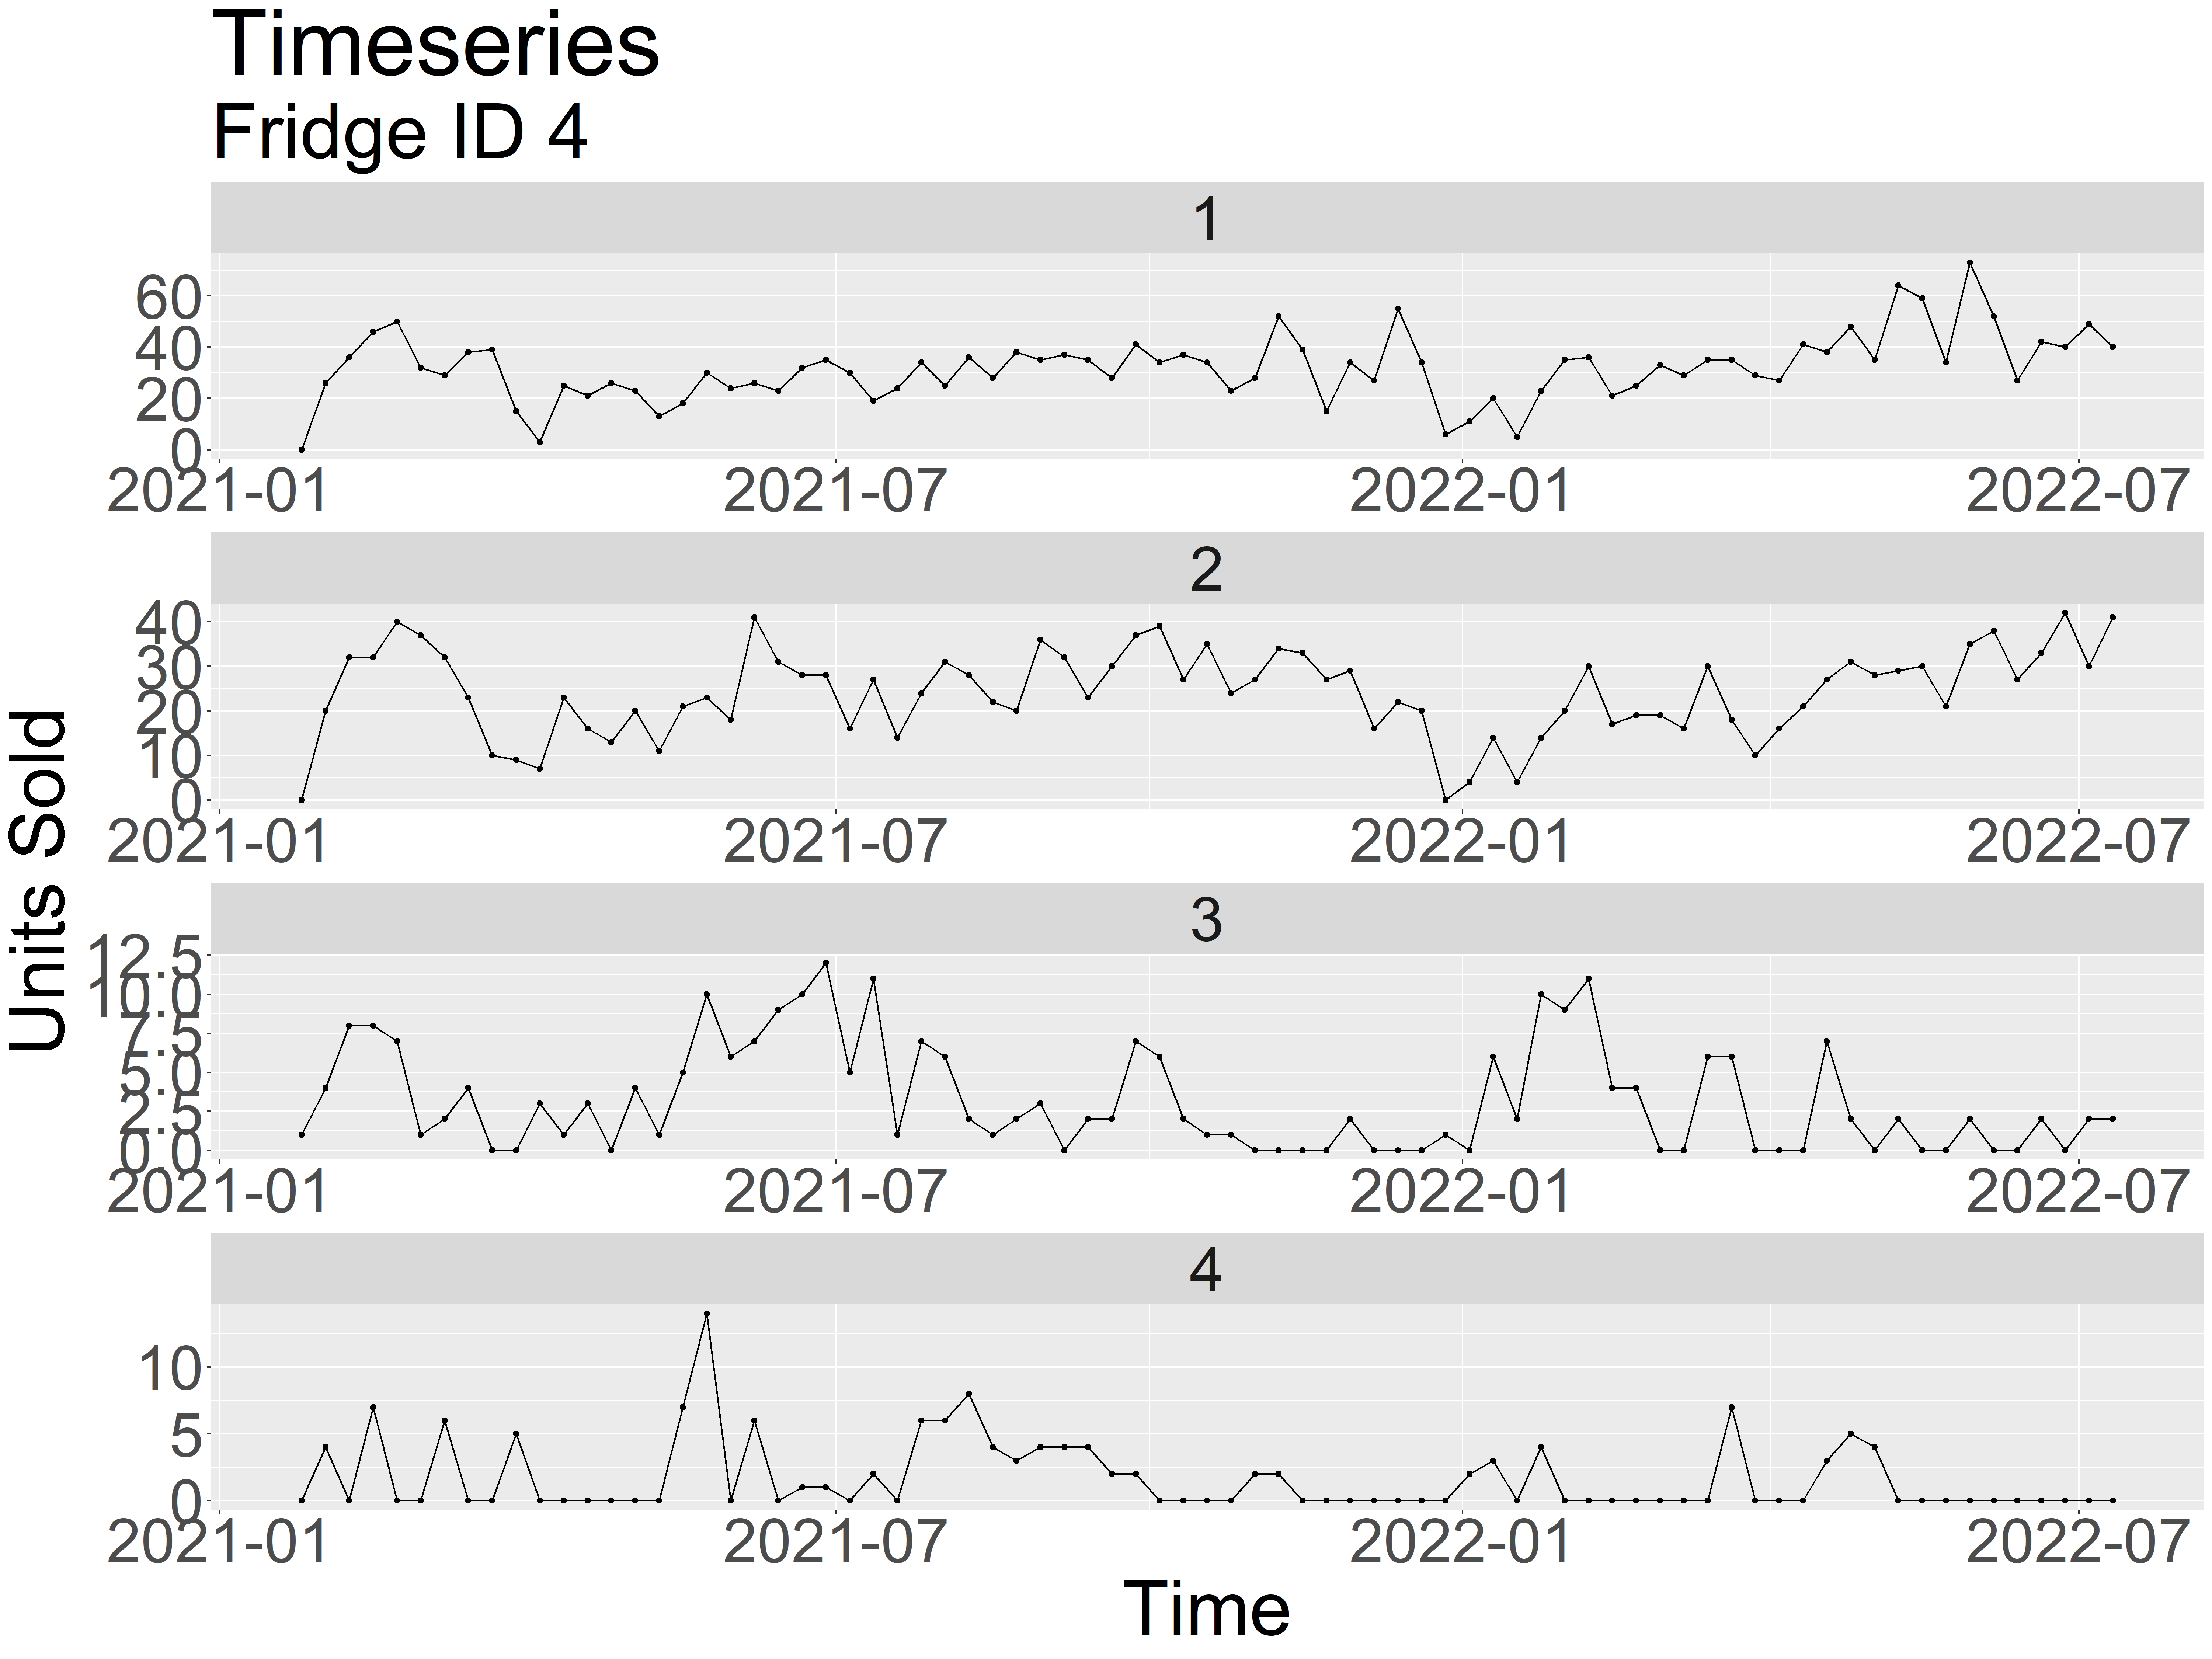
\includegraphics[width=\textwidth]{F:/Uni/Masterarbeit/Master-Thesis_git/Arbeit/Graphiken/Raw_Timeseries_ID4.png}
\caption{Fridge 4 with all four main categories}
\label{fig:TS Fridge 4}
\end{subfigure}
\hfill
\begin{subfigure}[b]{0.45\textwidth}
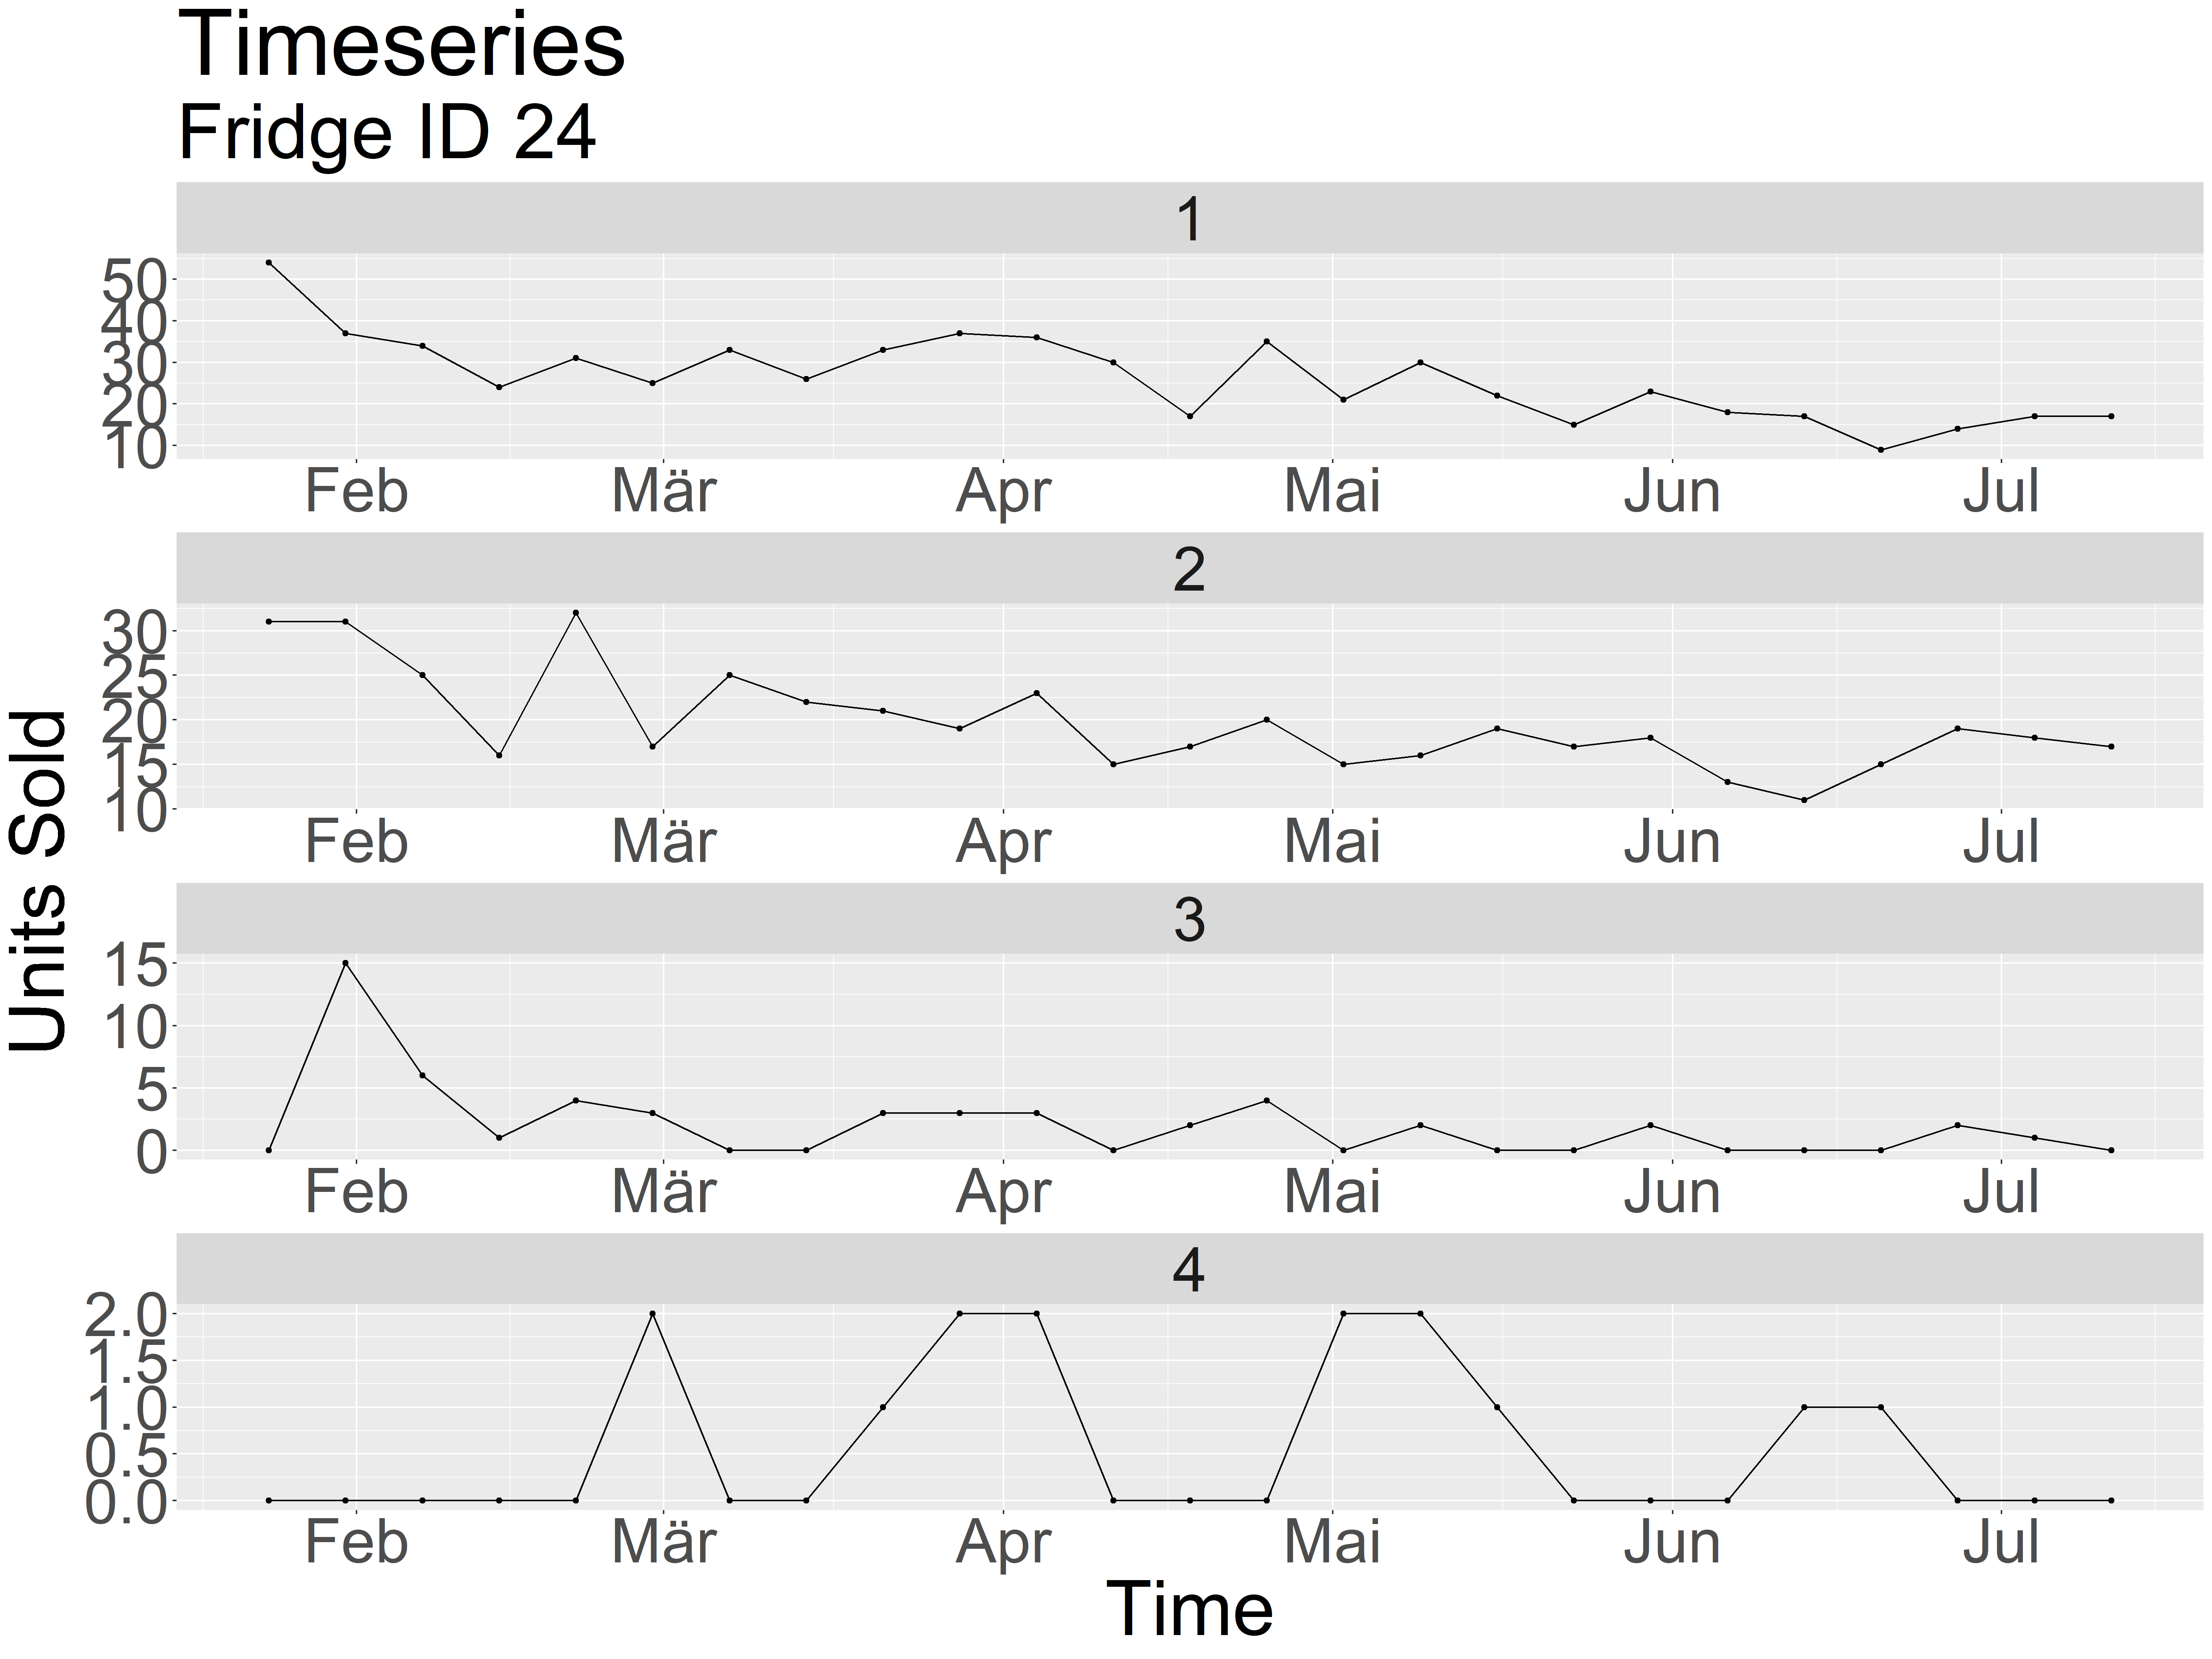
\includegraphics[width=\textwidth]{F:/Uni/Masterarbeit/Master-Thesis_git/Arbeit/Graphiken/Raw_Timeseries_ID24.png}
\caption{Fridge 24 with all four main categories}
\label{fig:TS Fridge 24}
\end{subfigure}
\caption{Timeseries for two fridges}
\label{fig:TS raw}
\end{figure}


The two plots in \ref{fig:TS raw} are good examples of the composition of our data. The scales of the sold units within a fridge vary widely. For example in figure \ref{fig:TS Fridge 24} the values for category 1 vary from above 50 to as low as 10, while for category 4 we only have values in the range of 0 to 2. In both figures \ref{fig:TS raw} for category 4, we can see the excessive amount of zero values in our data which makes the previously mentioned transformations necessary. 

Next in figure \ref{fig:TS Coda}, we add the predictions of the CoDA model. For this model we used the whole history and half of the data for the window length. In addition we extend the window at every time point, add 0.5 to all values and use the one-vs-all method. We can see that this captures the general trend well however, struggles with unexpected high peaks. In addition it is able to handle the difference in scales as seen in \ref{fig:Coda Fridge 4}. Both, categories 1 and 2 with bigger values and categories 3 and 4 with lower values, are in general modelled well. Also in timeseries with less data available, as in fridge 24 \ref{fig:Coda Fridge 24}, the model works well. Especially category 3 with its low values is predicted well. 

\begin{figure}[htb]
\centering
\begin{subfigure}[b]{0.45\textwidth}
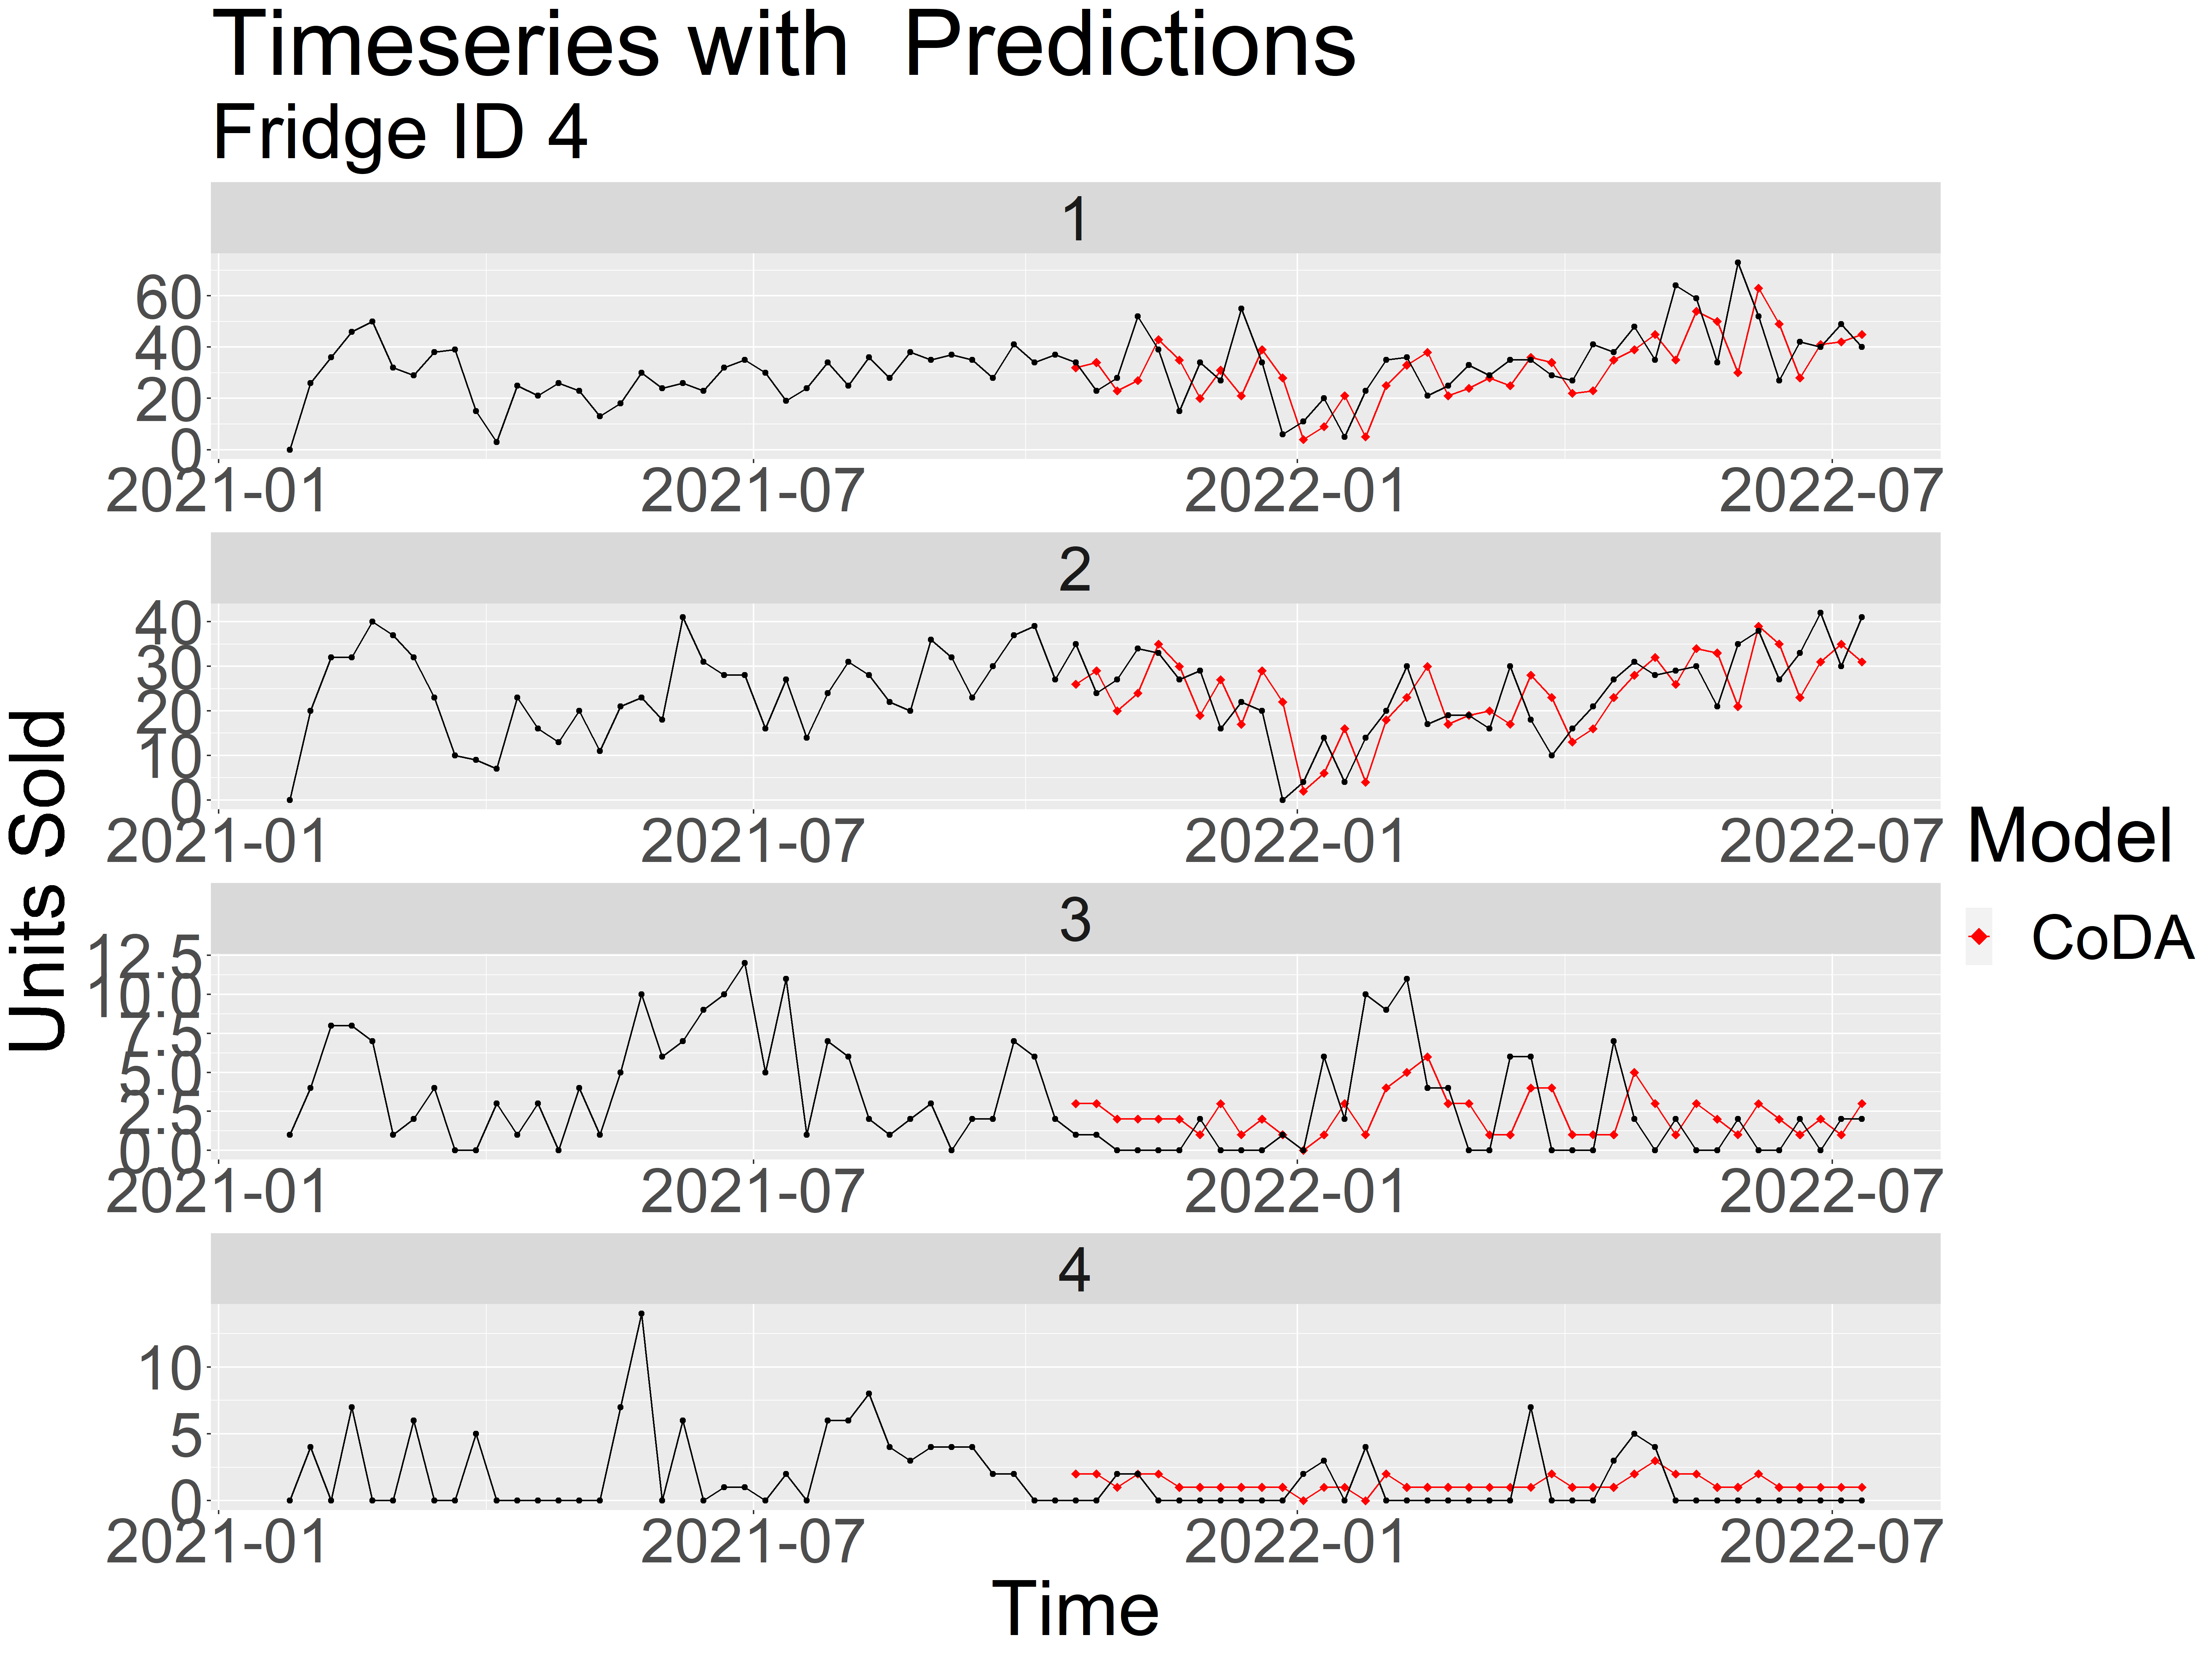
\includegraphics[width=\textwidth]{F:/Uni/Masterarbeit/Master-Thesis_git/Arbeit/Graphiken/Coda_Timeseries_ID4.png}
\caption{Fridge 4 with the CoDA model}
\label{fig:Coda Fridge 4}
\end{subfigure}
\hfill
\begin{subfigure}[b]{0.45\textwidth}
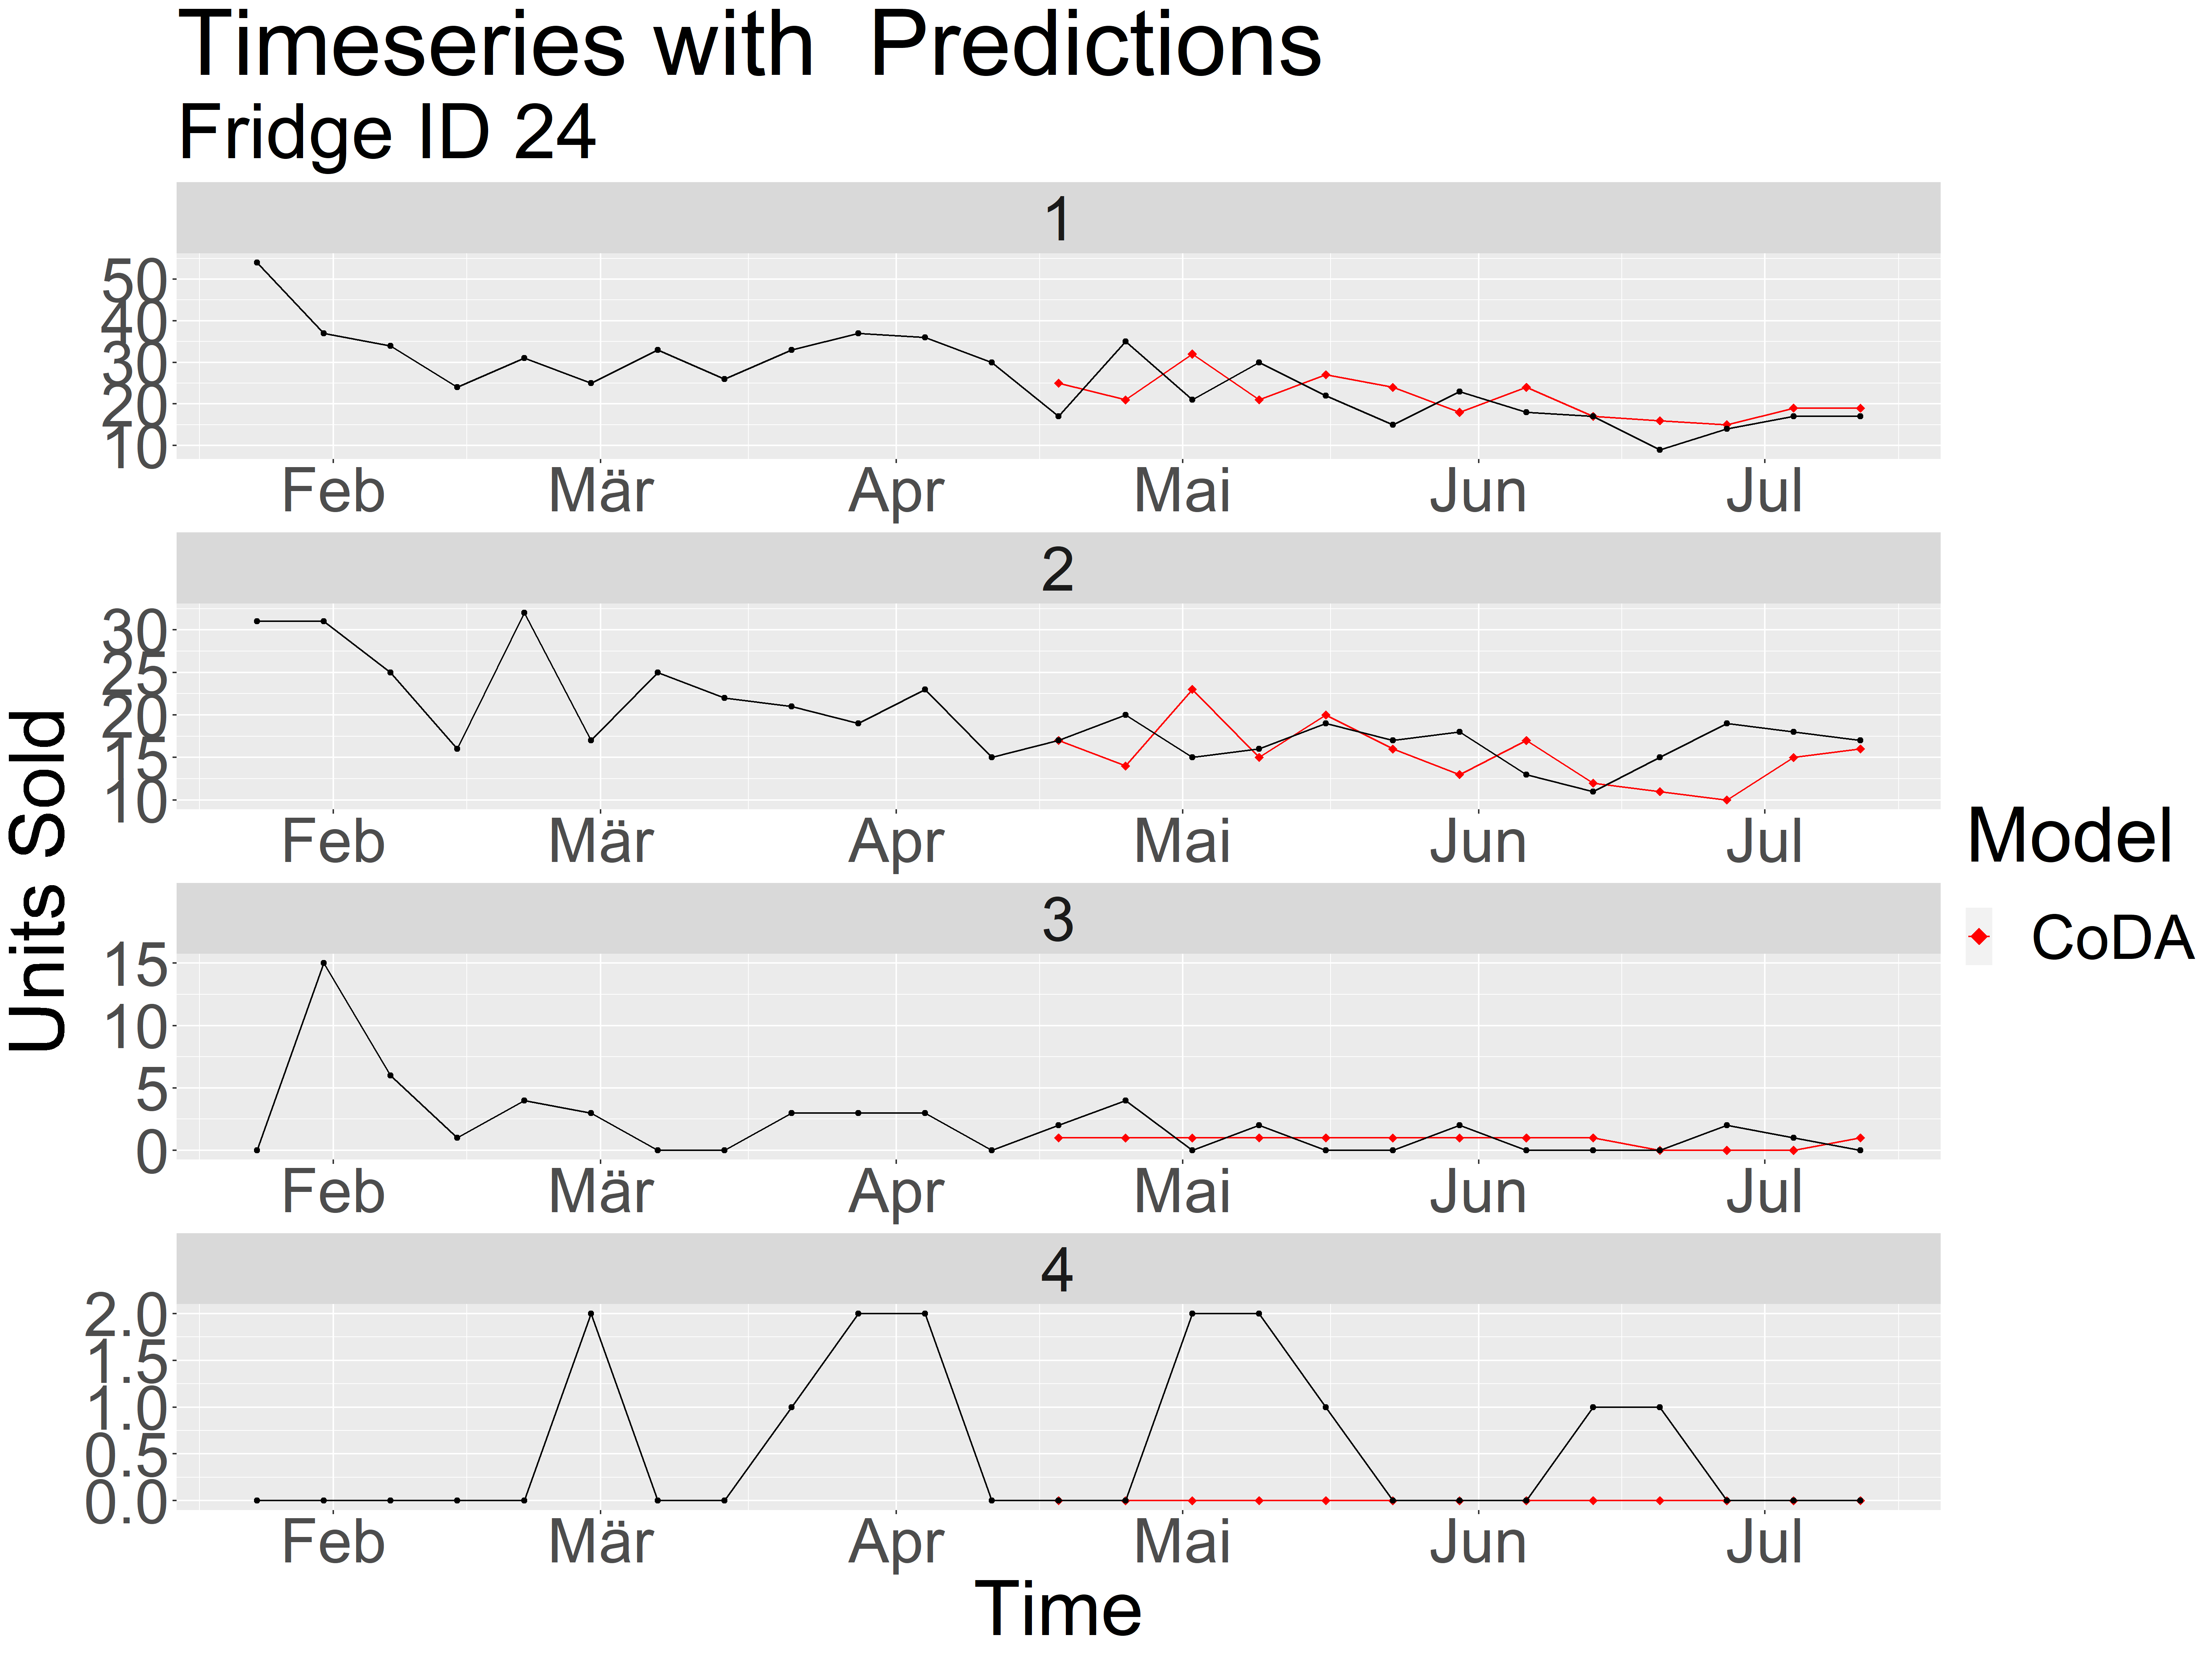
\includegraphics[width=\textwidth]{F:/Uni/Masterarbeit/Master-Thesis_git/Arbeit/Graphiken/Coda_Timeseries_ID24.png}
\caption{Fridge 24 with the CoDA model}
\label{fig:Coda Fridge 24}
\end{subfigure}
\caption{Timeseries with CoDA model}
\label{fig:TS Coda}
\end{figure}



In figure \ref{fig:TS Ingarch} we apply the INGARCH model to the timeseries. For this, we used the whole history, half of the data for the window length, extend the window at every time point, add one to all zero values and used the poisson distribution. We used no external factors and set $p=1, q=1$ in model \ref{eq:Ingarch model with external effect}. The general trend is again captured well and in the instance of \ref{fig:Ingarch Fridge 4} it seems to be more reactive to sudden peaks, as often the value predicted after such a peak is heavily influenced by it.

\begin{figure}[htb]
\centering
\begin{subfigure}[b]{0.45\textwidth}
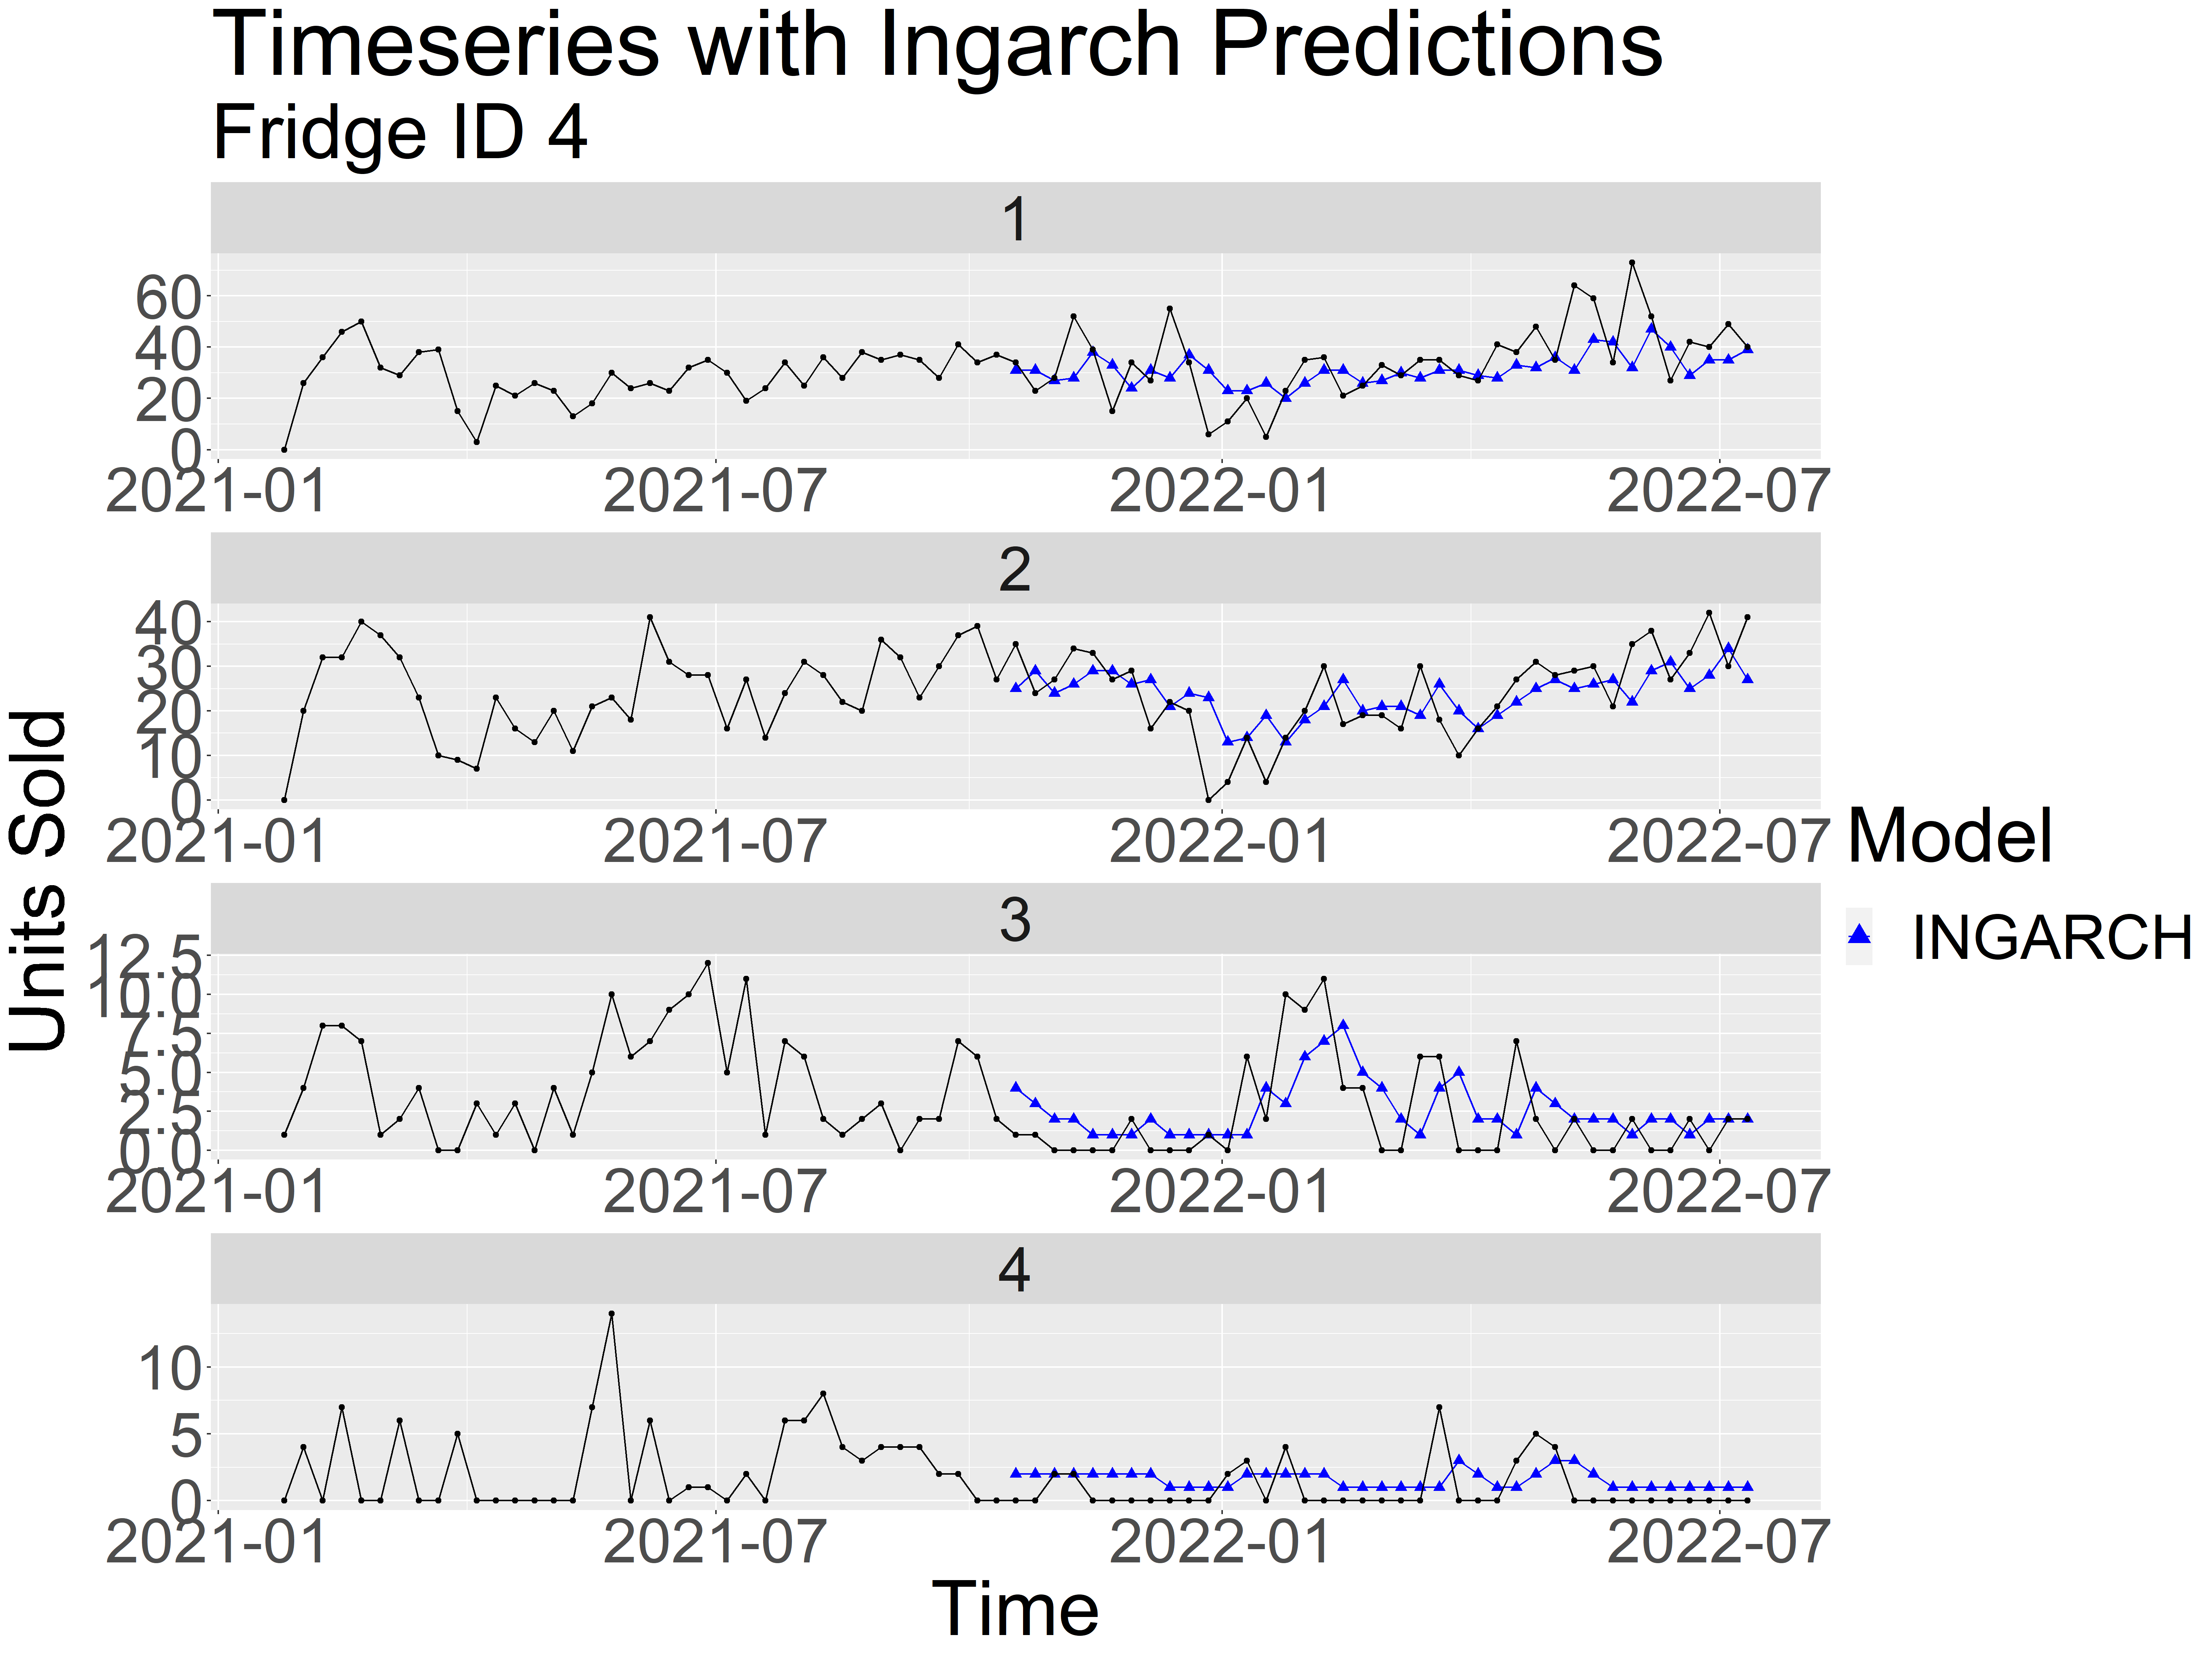
\includegraphics[width=\textwidth]{F:/Uni/Masterarbeit/Master-Thesis_git/Arbeit/Graphiken/Ingarch_Timeseries_ID4.png}
\caption{Fridge 4 with the INGARCH model}
\label{fig:Ingarch Fridge 4}
\end{subfigure}
\hfill
\begin{subfigure}[b]{0.45\textwidth}
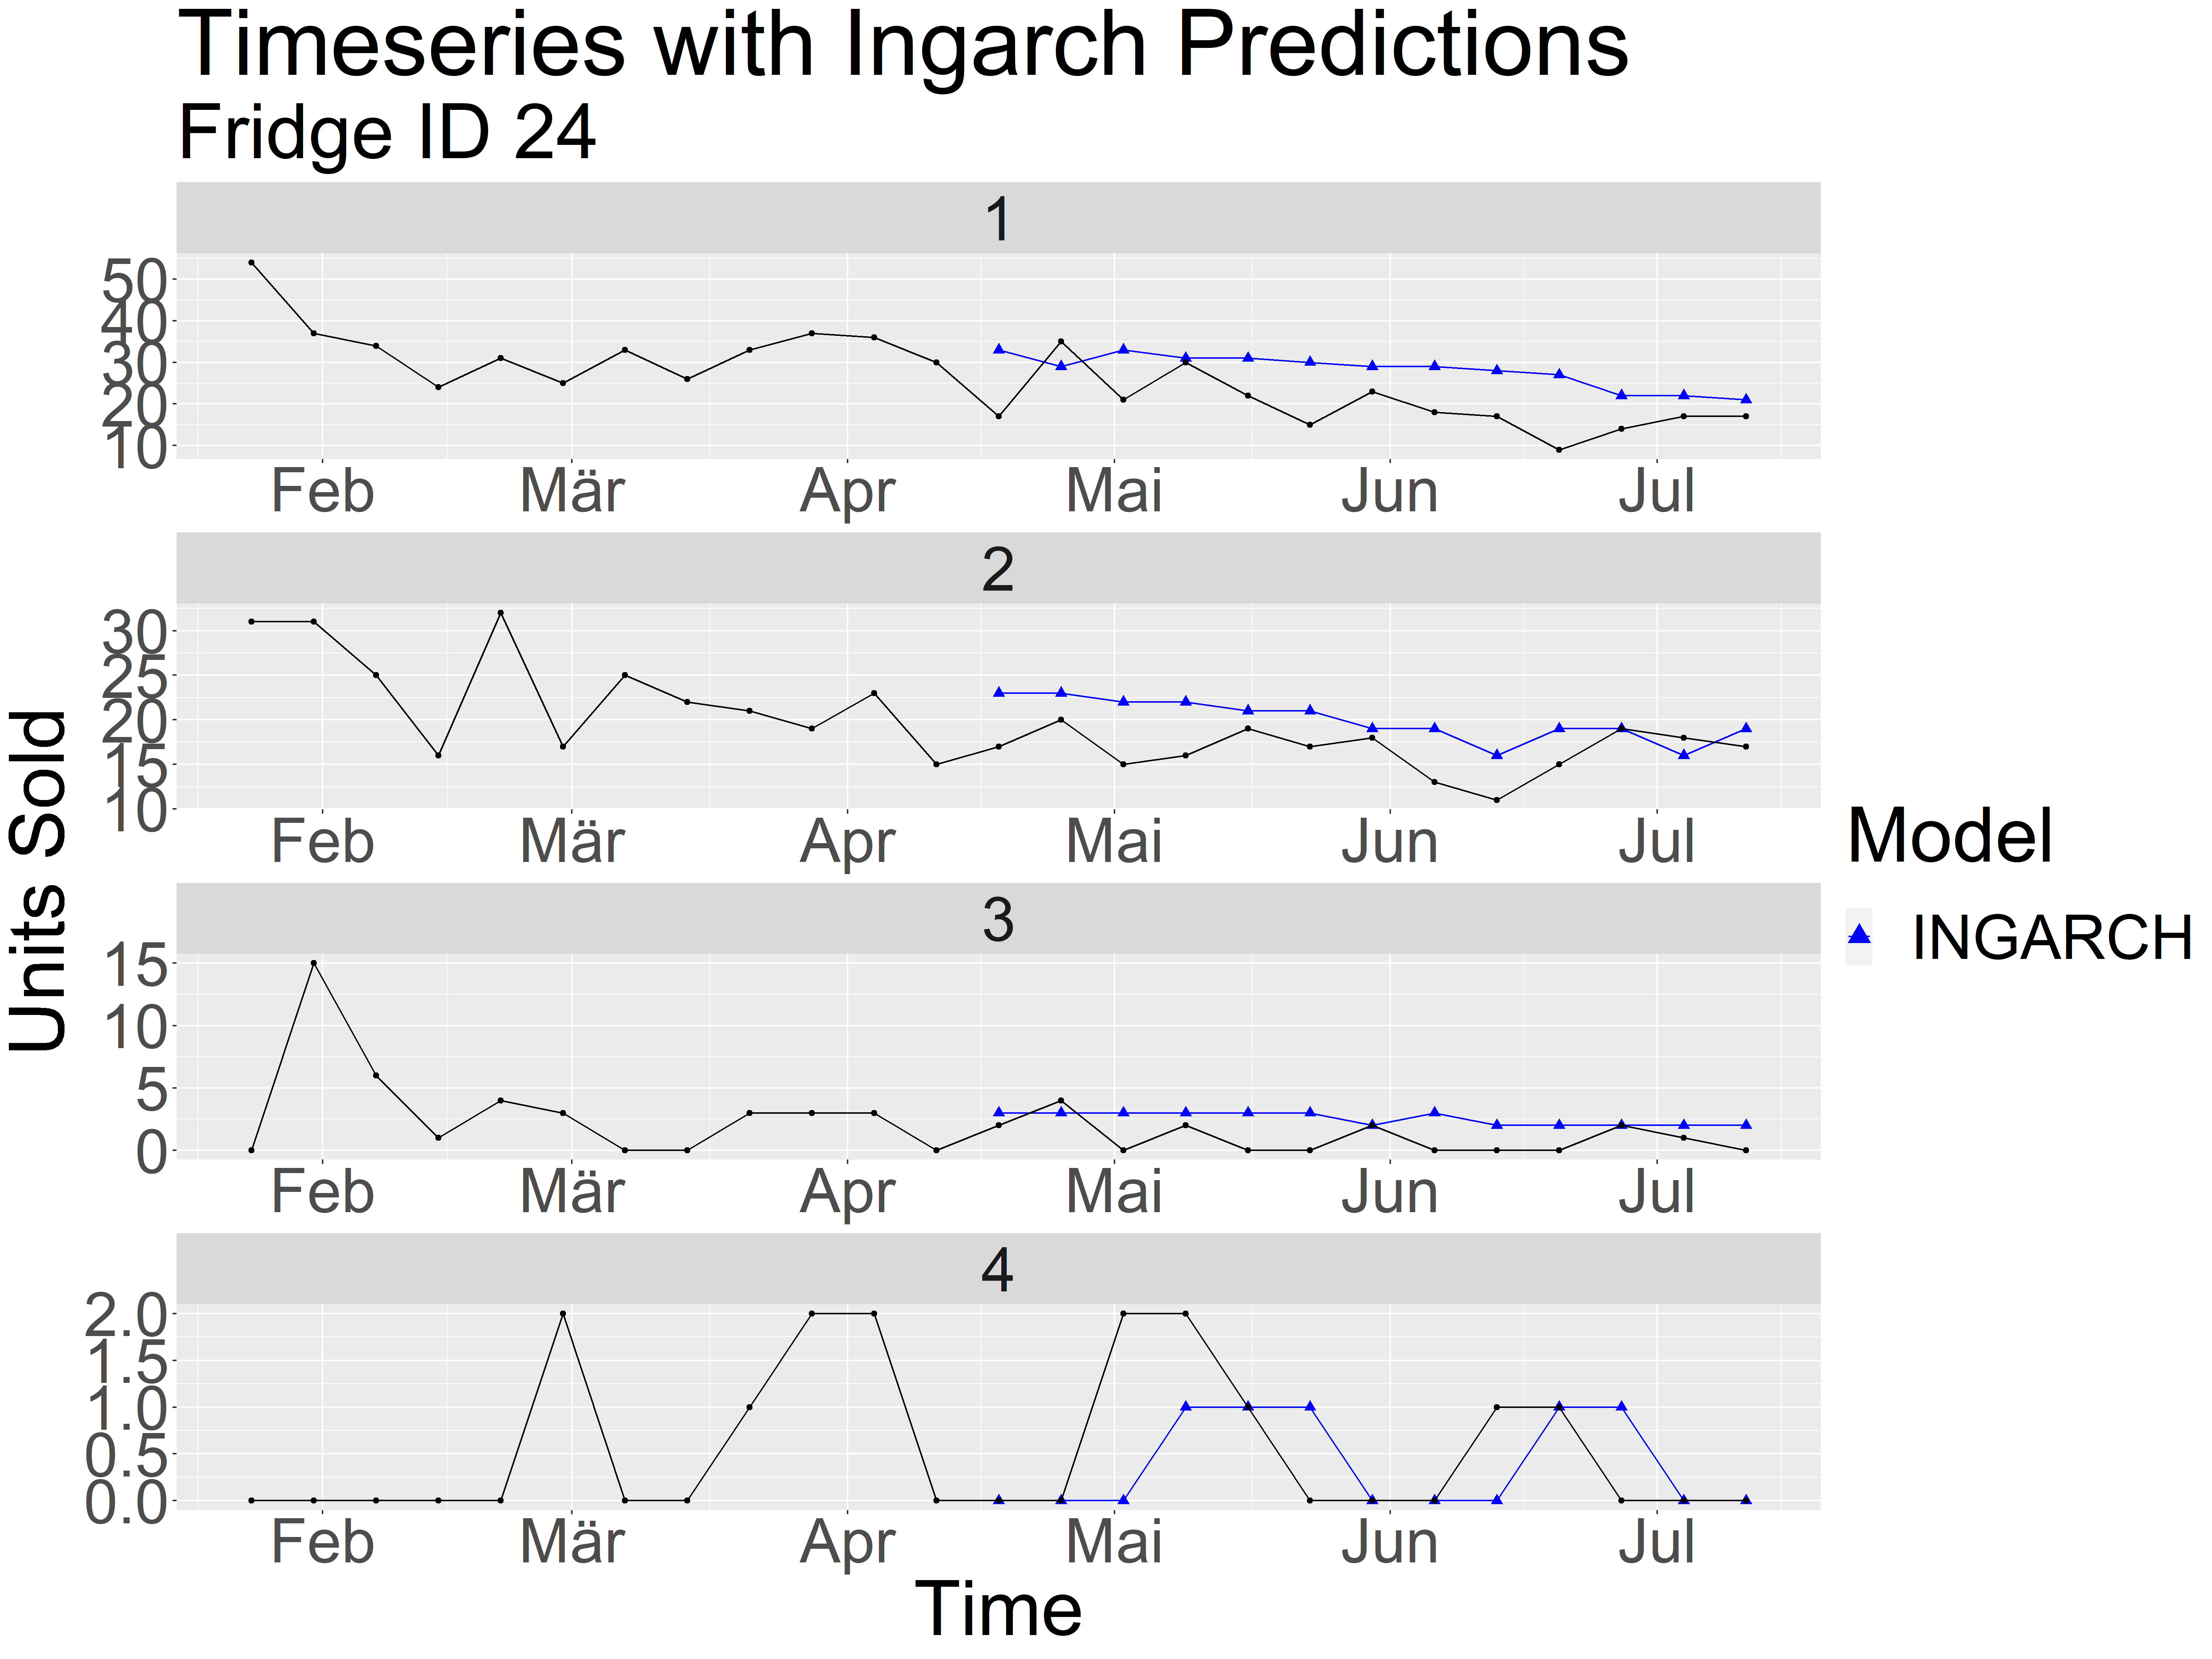
\includegraphics[width=\textwidth]{F:/Uni/Masterarbeit/Master-Thesis_git/Arbeit/Graphiken/Ingarch_Timeseries_ID24.png}
\caption{Fridge 24 with the INGARCH model}
\label{fig:Ingarch Fridge 24}
\end{subfigure}
\caption{Timeseries with INGARCH model}
\label{fig:TS Ingarch}
\end{figure}


To directly compare both models, we plot the predictions in one figure \ref{fig:TS Both}. The model specifications are the same as above. We can see that the models produce similar results to each other. In this instances it appears that INGARCH predicts slightly higher values than CoDA. 

\begin{figure}[htb]
\centering
\begin{subfigure}[b]{0.8\textwidth}
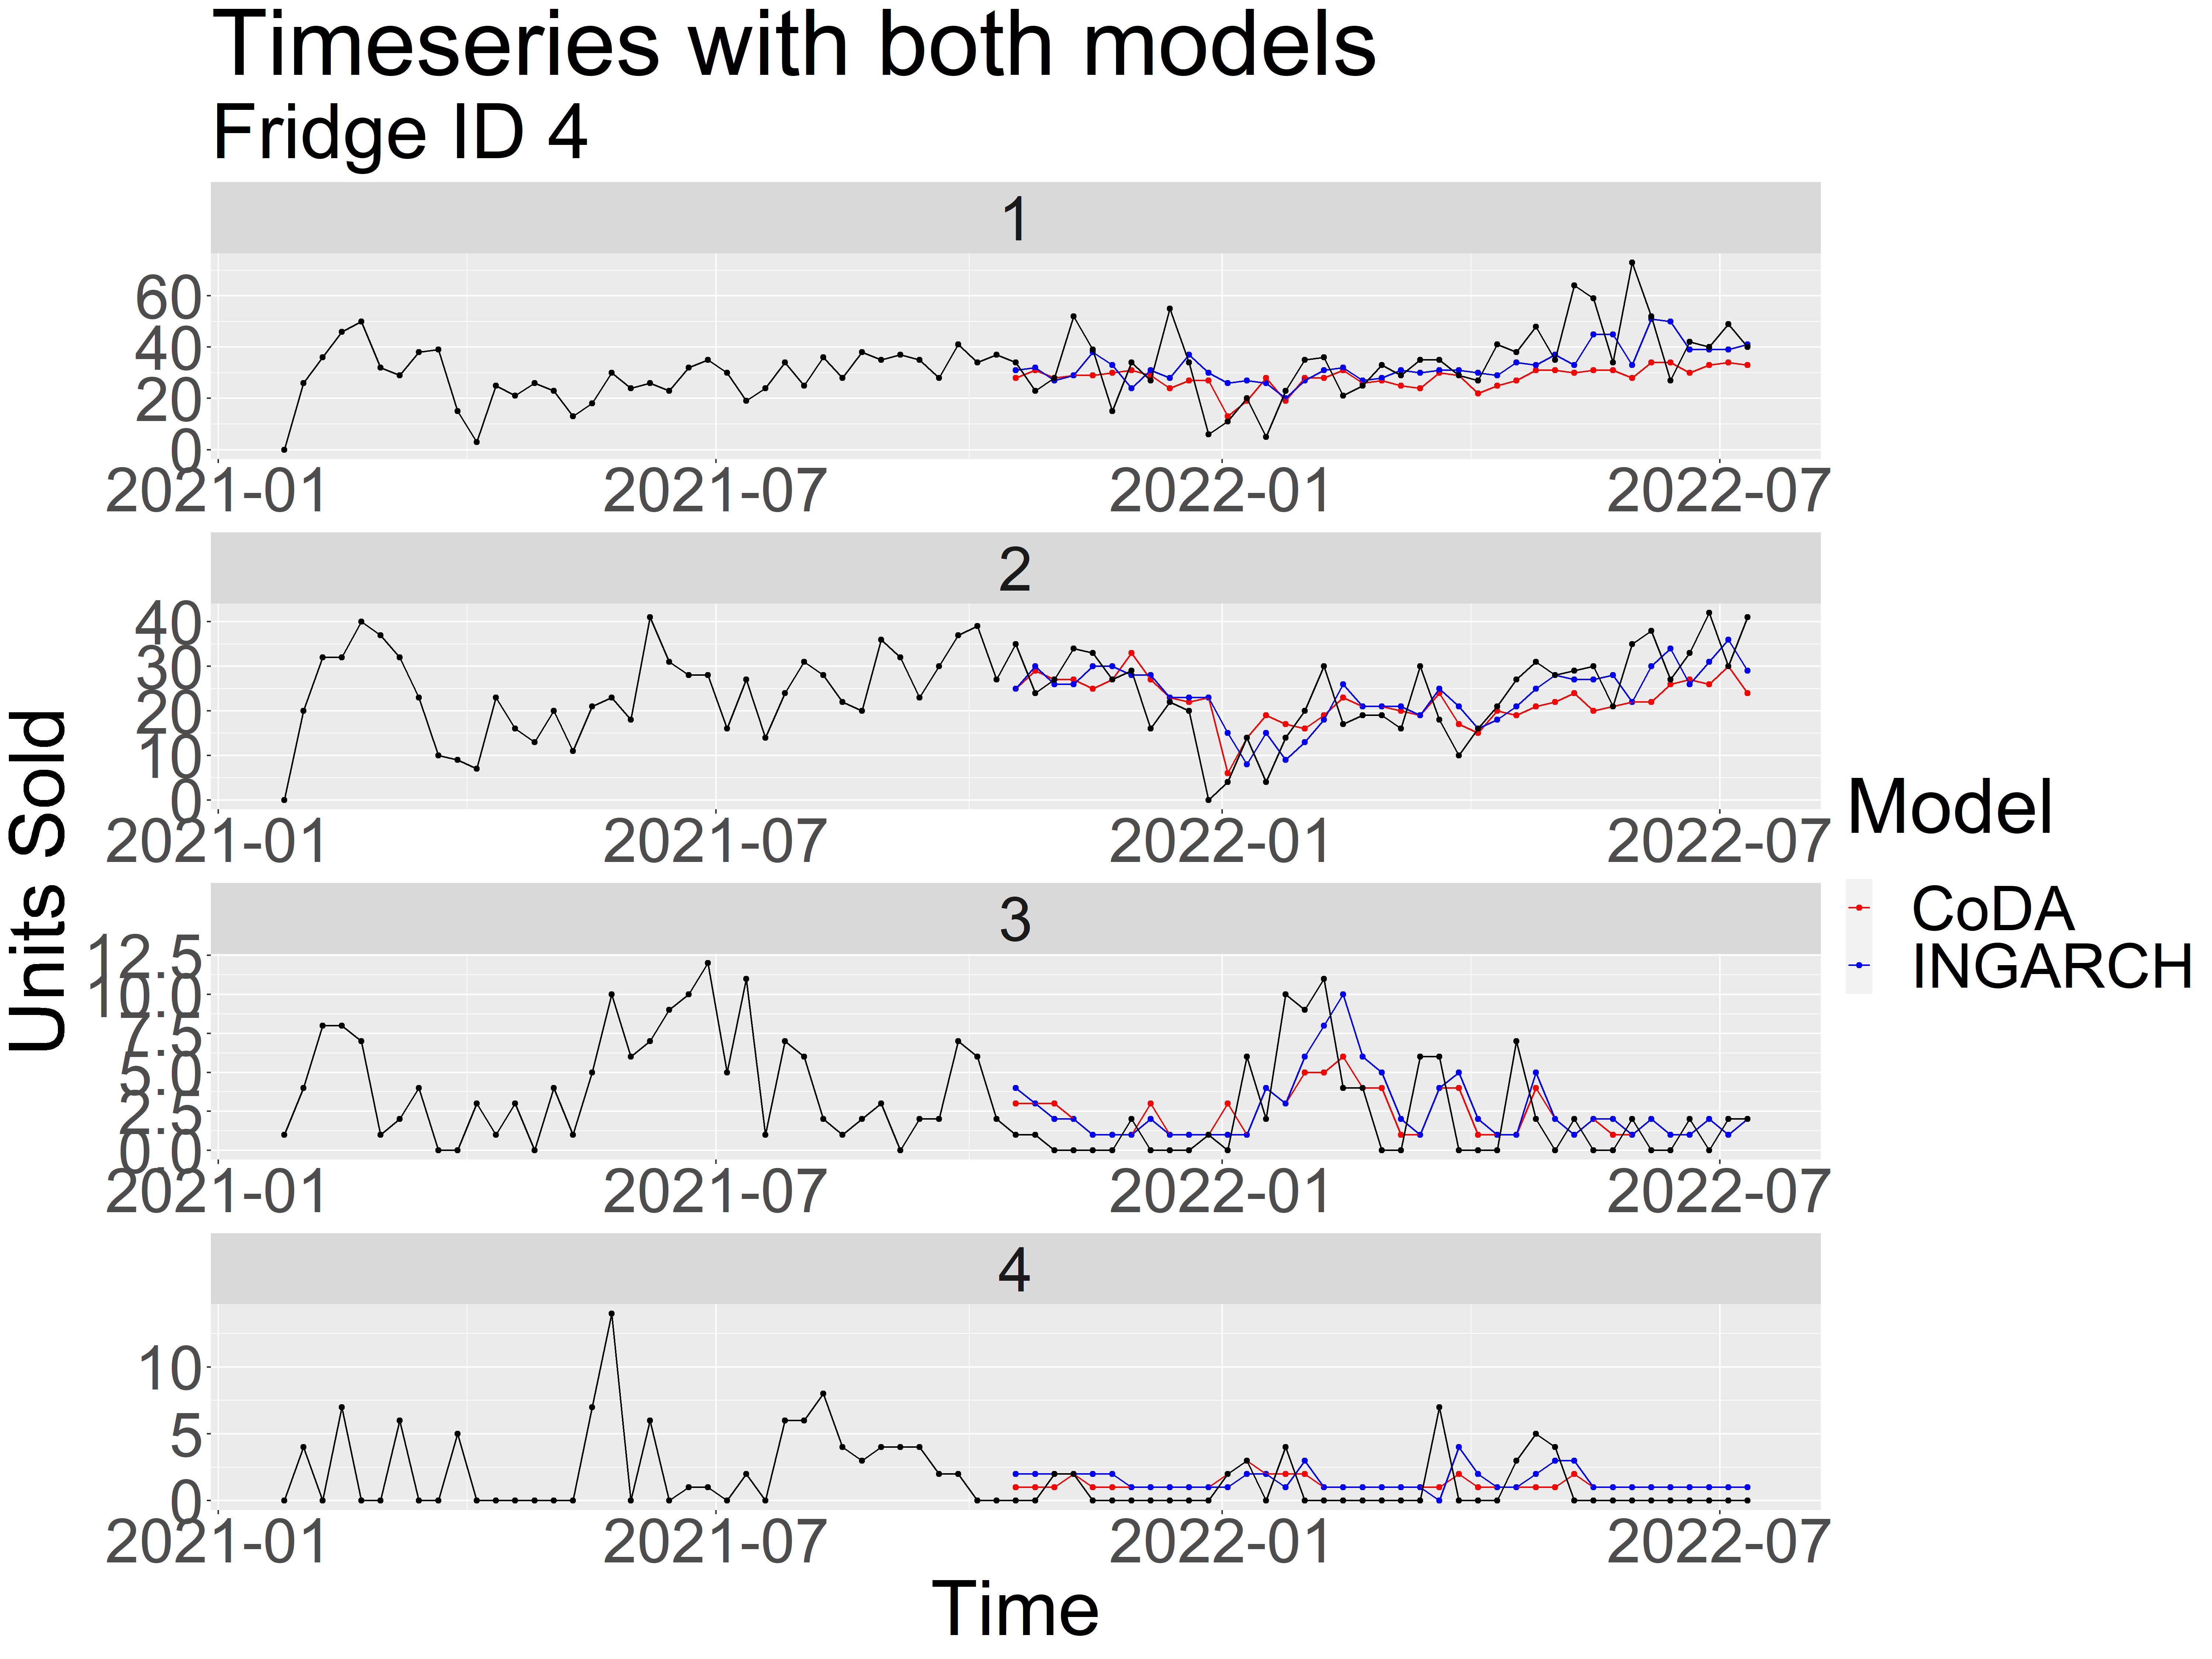
\includegraphics[width=\textwidth]{F:/Uni/Masterarbeit/Master-Thesis_git/Arbeit/Graphiken/Both_Timeseries_ID4.png}
\caption{Fridge 4 with the both models}
\label{fig:Both Fridge 4}
\end{subfigure}
\hfill
\begin{subfigure}[b]{0.8\textwidth}
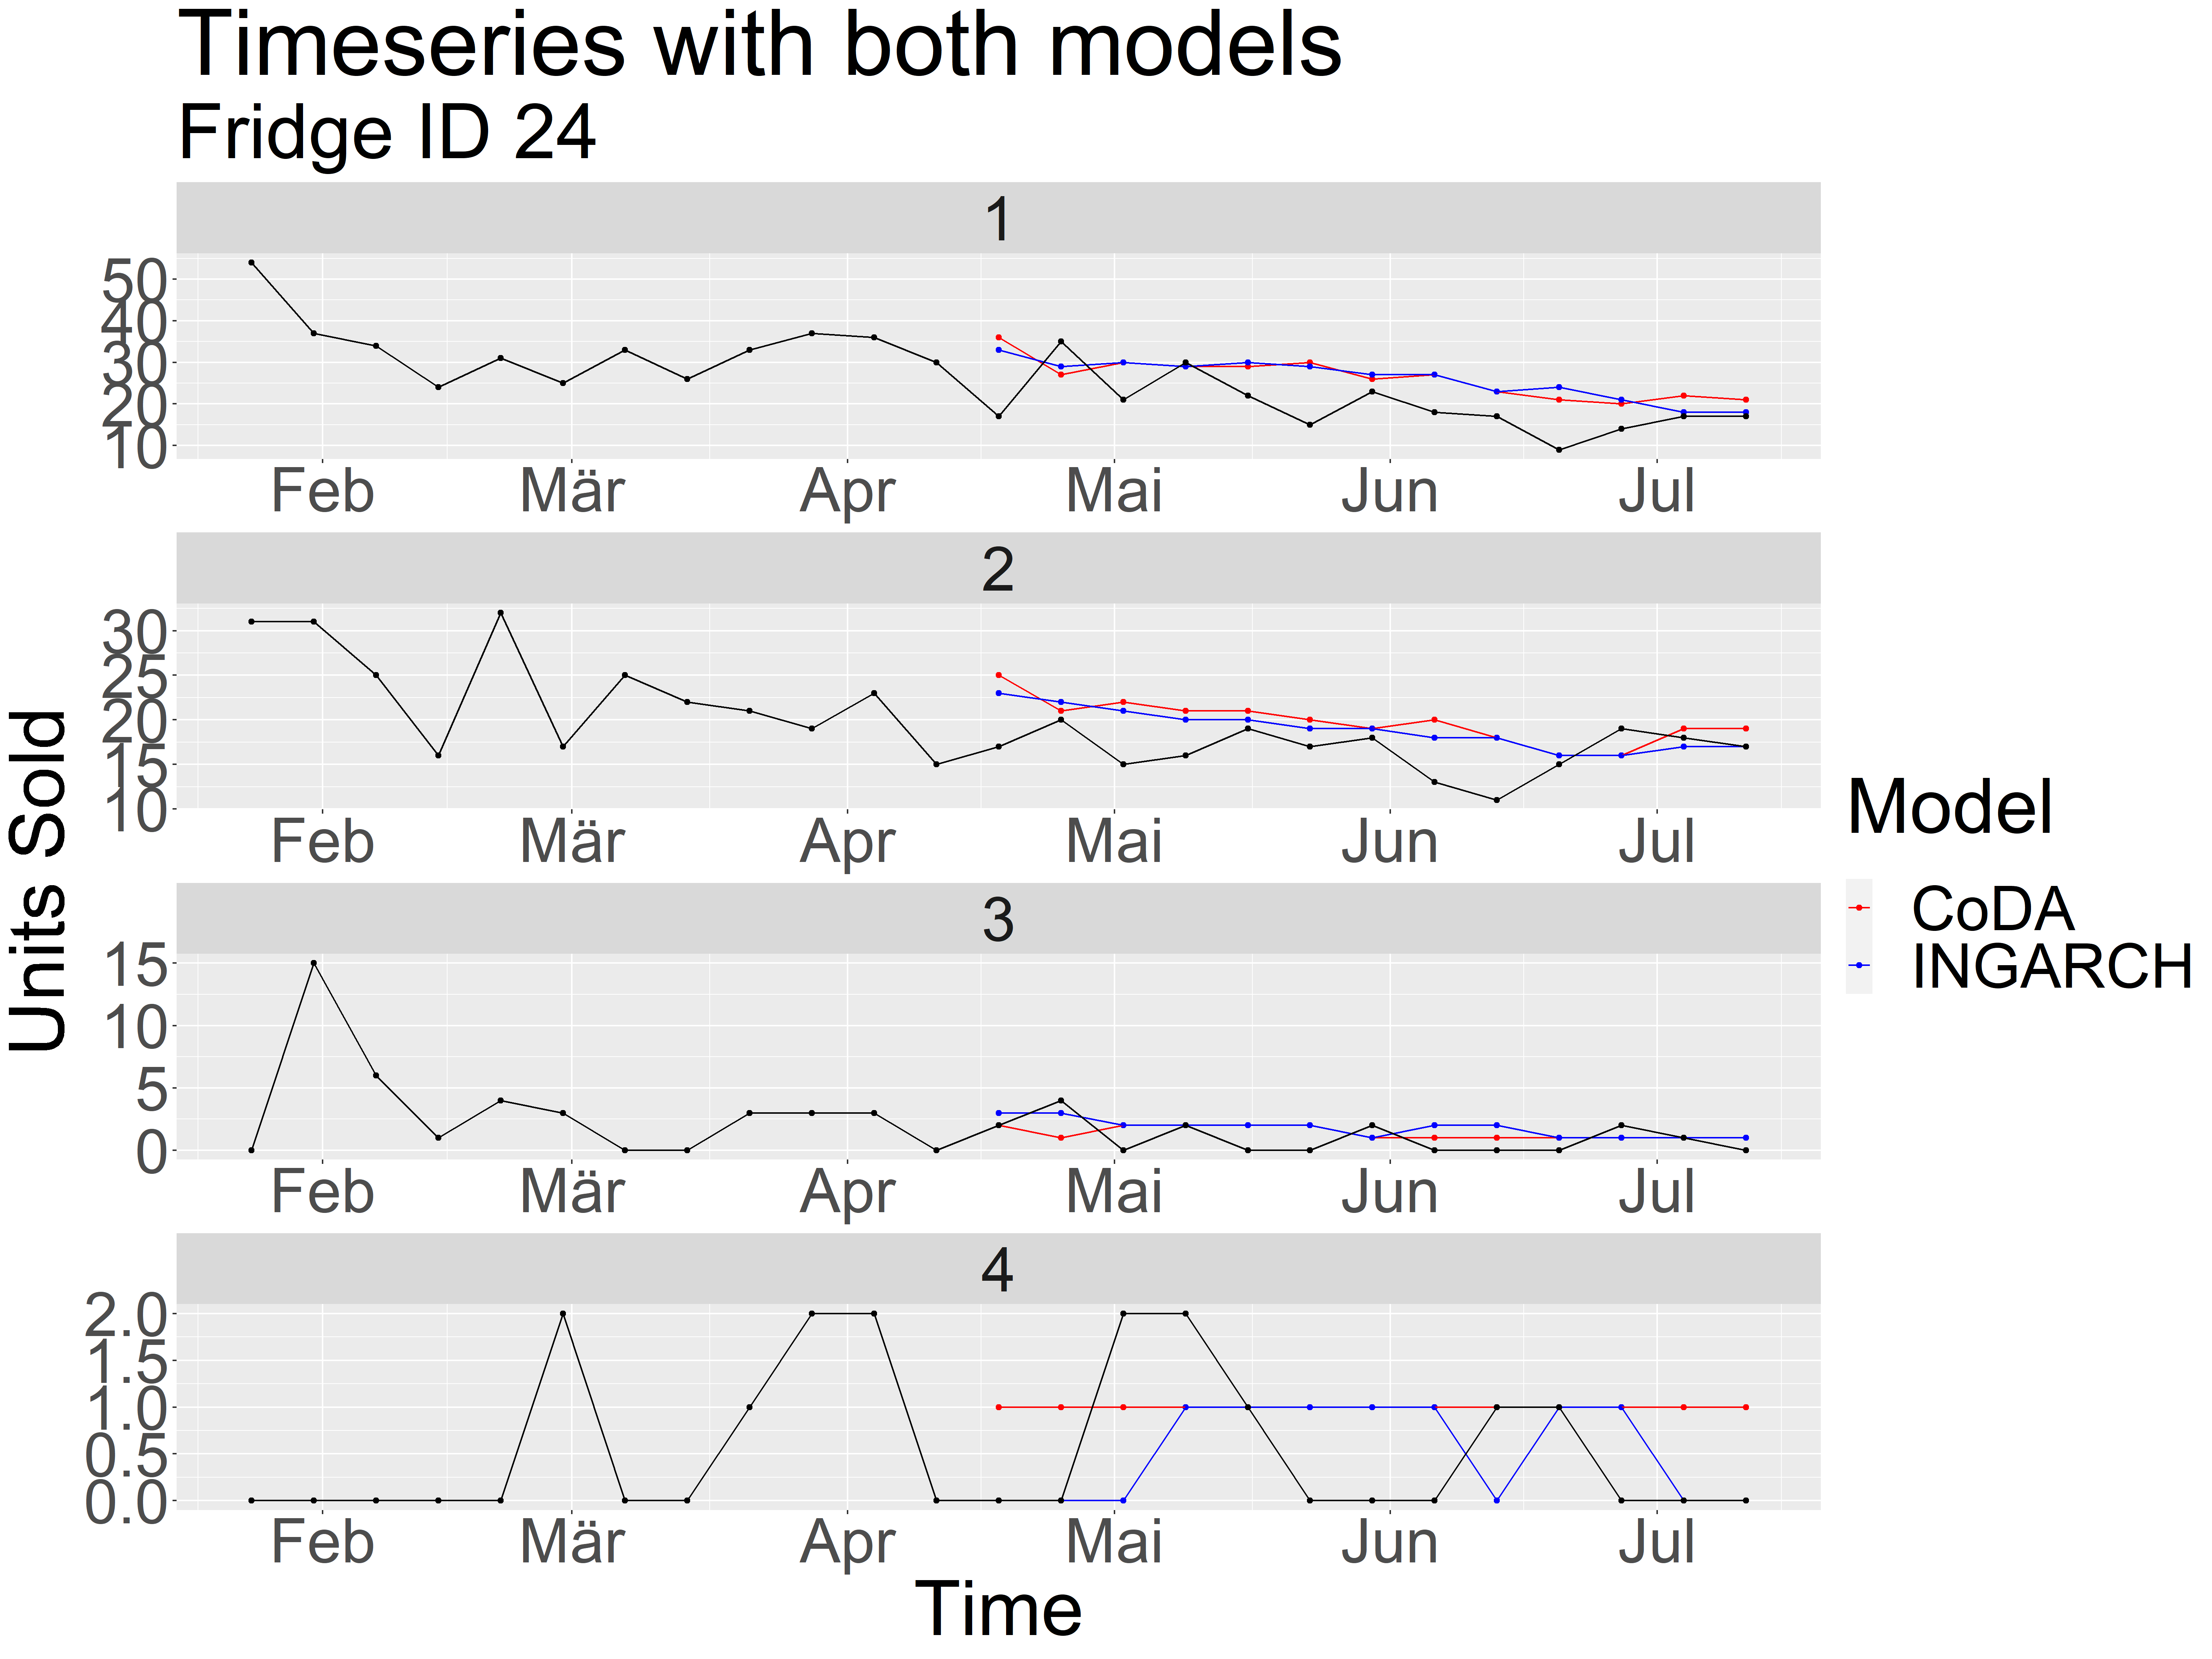
\includegraphics[width=\textwidth]{F:/Uni/Masterarbeit/Master-Thesis_git/Arbeit/Graphiken/Both_Timeseries_ID24.png}
\caption{Fridge 24 with the both models}
\label{fig:Both Fridge 24}
\end{subfigure}
\caption{Timeseries with both models}
\label{fig:TS Both}
\end{figure}


In order to get some further insight in the accuracy of our predictions, we added 95 \% prediction intervals \ref{fig:TS BothPI}. Here we can see some differences between the intervals. While for categories with bigger values the bands are quite similar in width, for categories with lower values, CoDA has much wider bands. This is especially visible in \ref{fig:BothPI Fridge 4} for category 3 and 4. However, most data points are covered by both bands.
\begin{figure}[htb]
\centering
\begin{subfigure}[b]{0.8\textwidth}
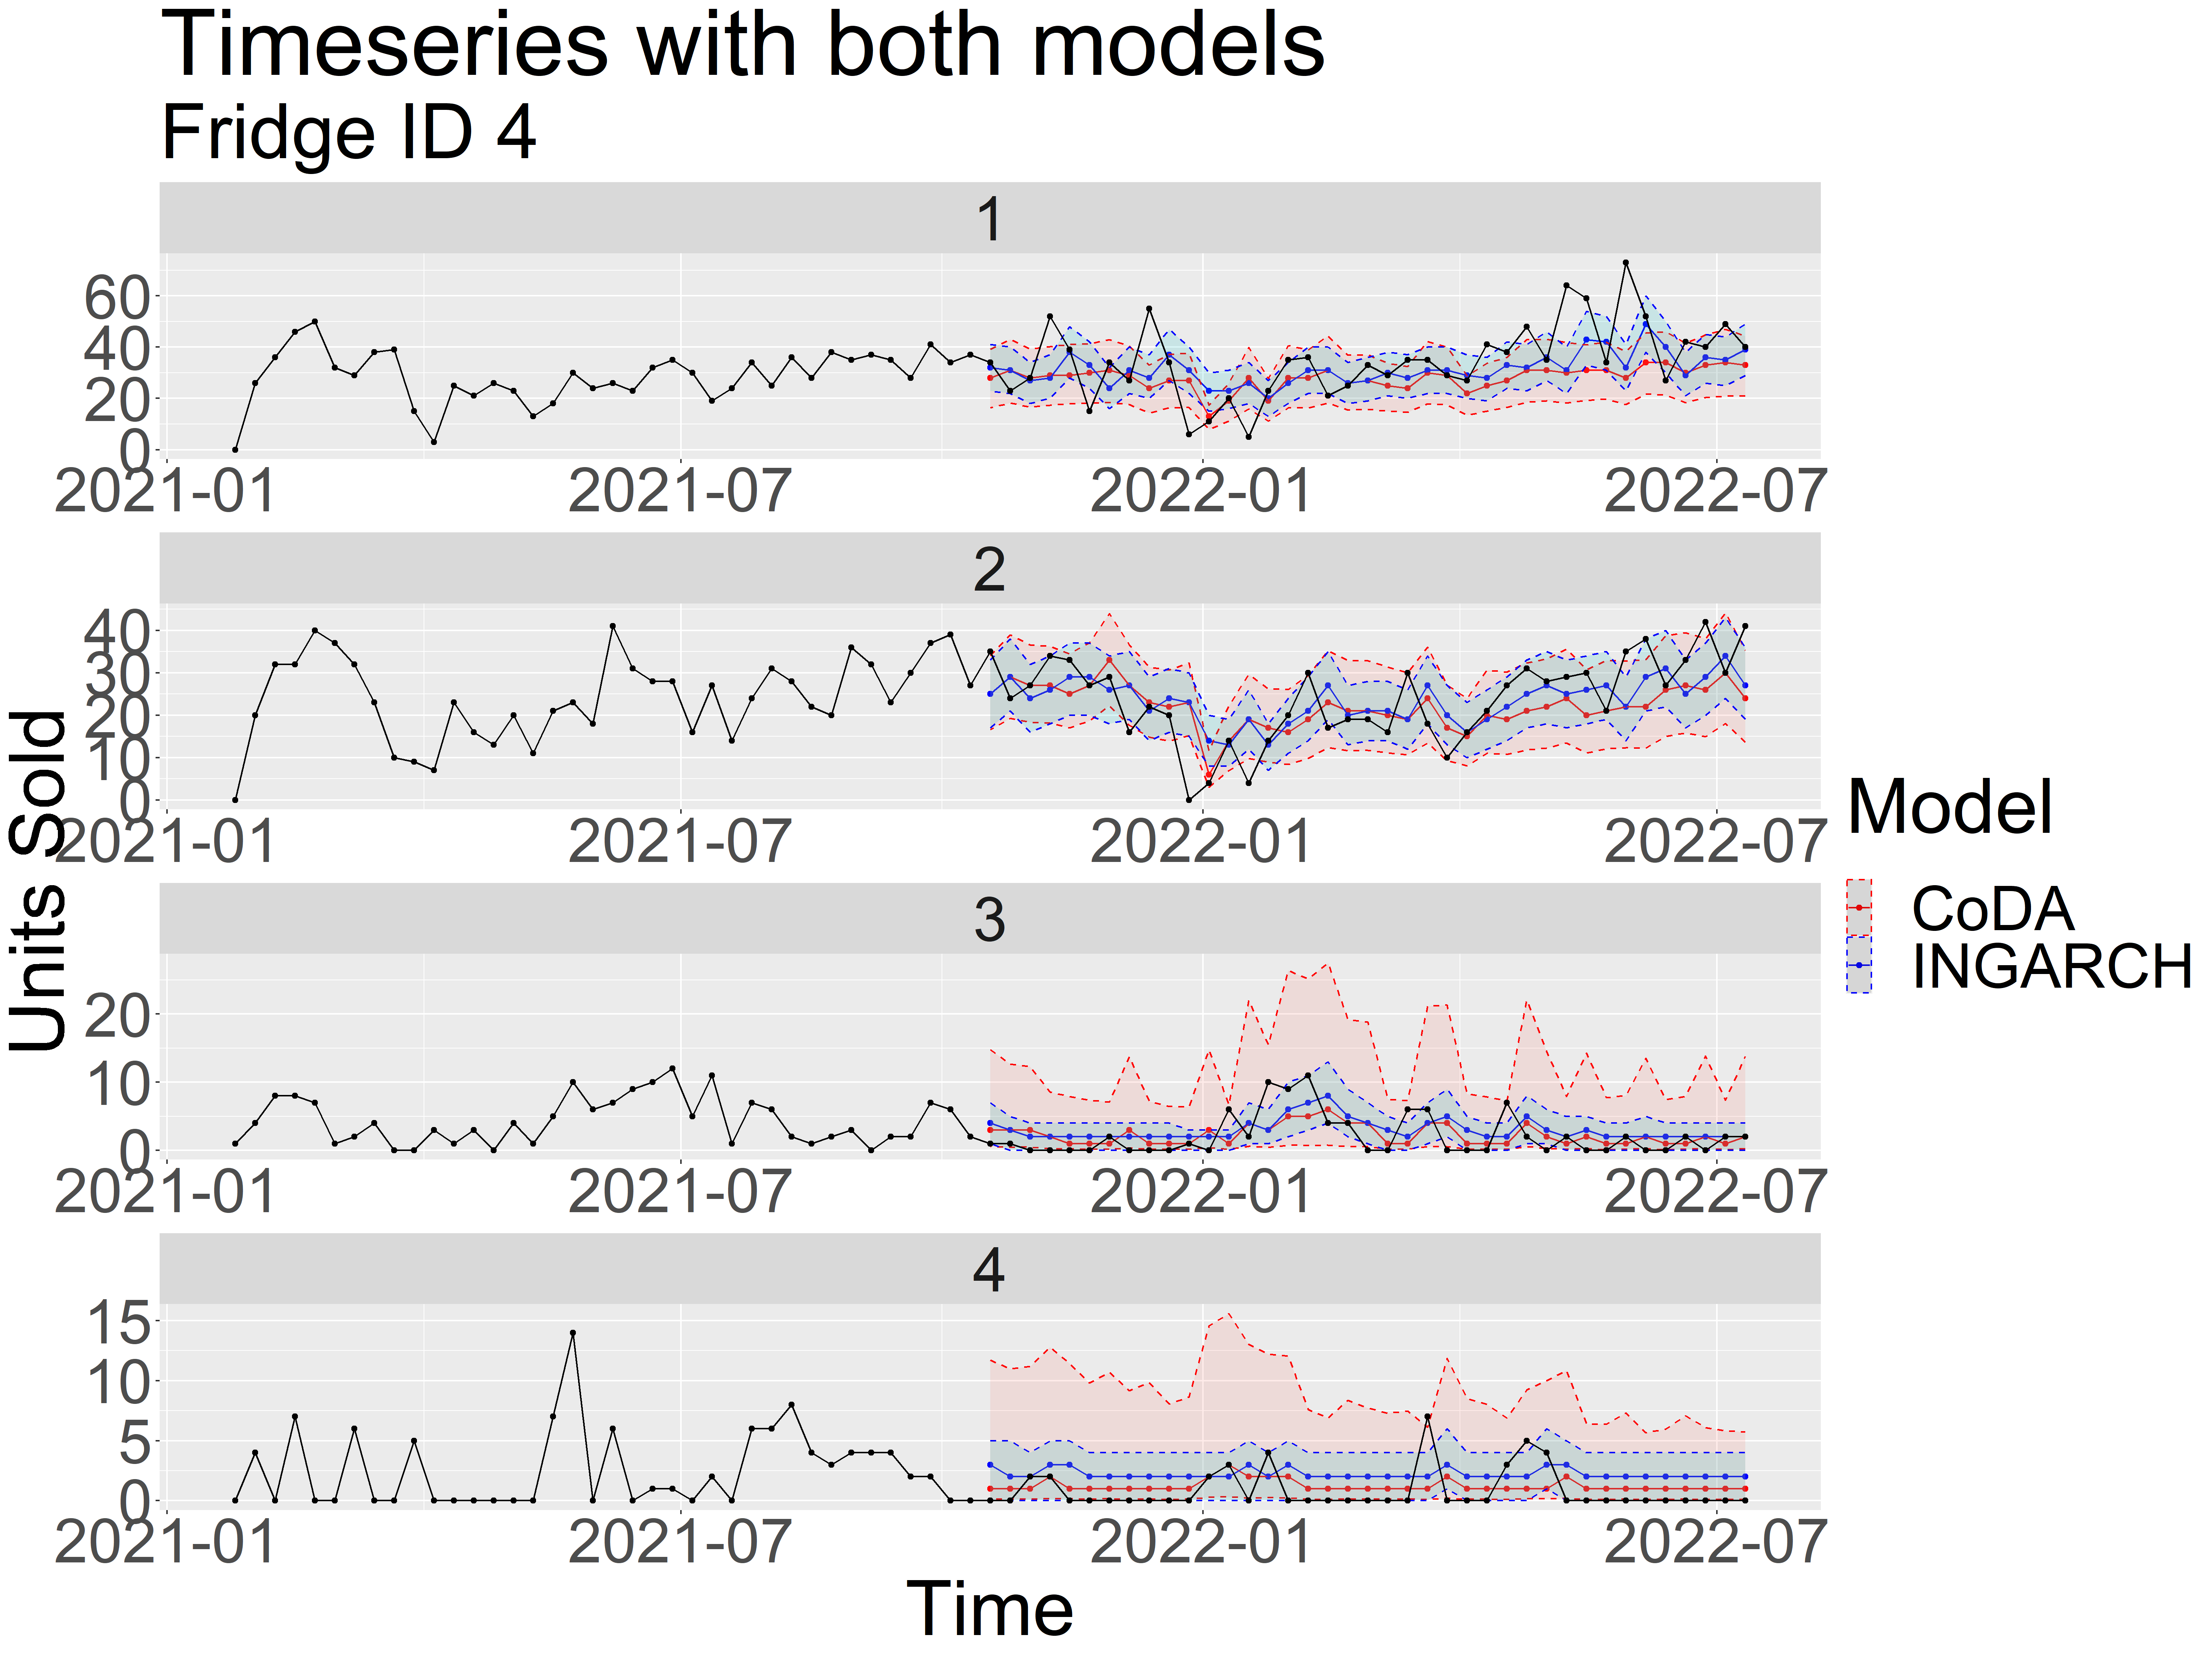
\includegraphics[width=\textwidth]{F:/Uni/Masterarbeit/Master-Thesis_git/Arbeit/Graphiken/BothPI_Timeseries_ID4.png}
\caption{Fridge 4 with the both models and their prediction intervals}
\label{fig:BothPI Fridge 4}
\end{subfigure}
\hfill
\begin{subfigure}[b]{0.8\textwidth}
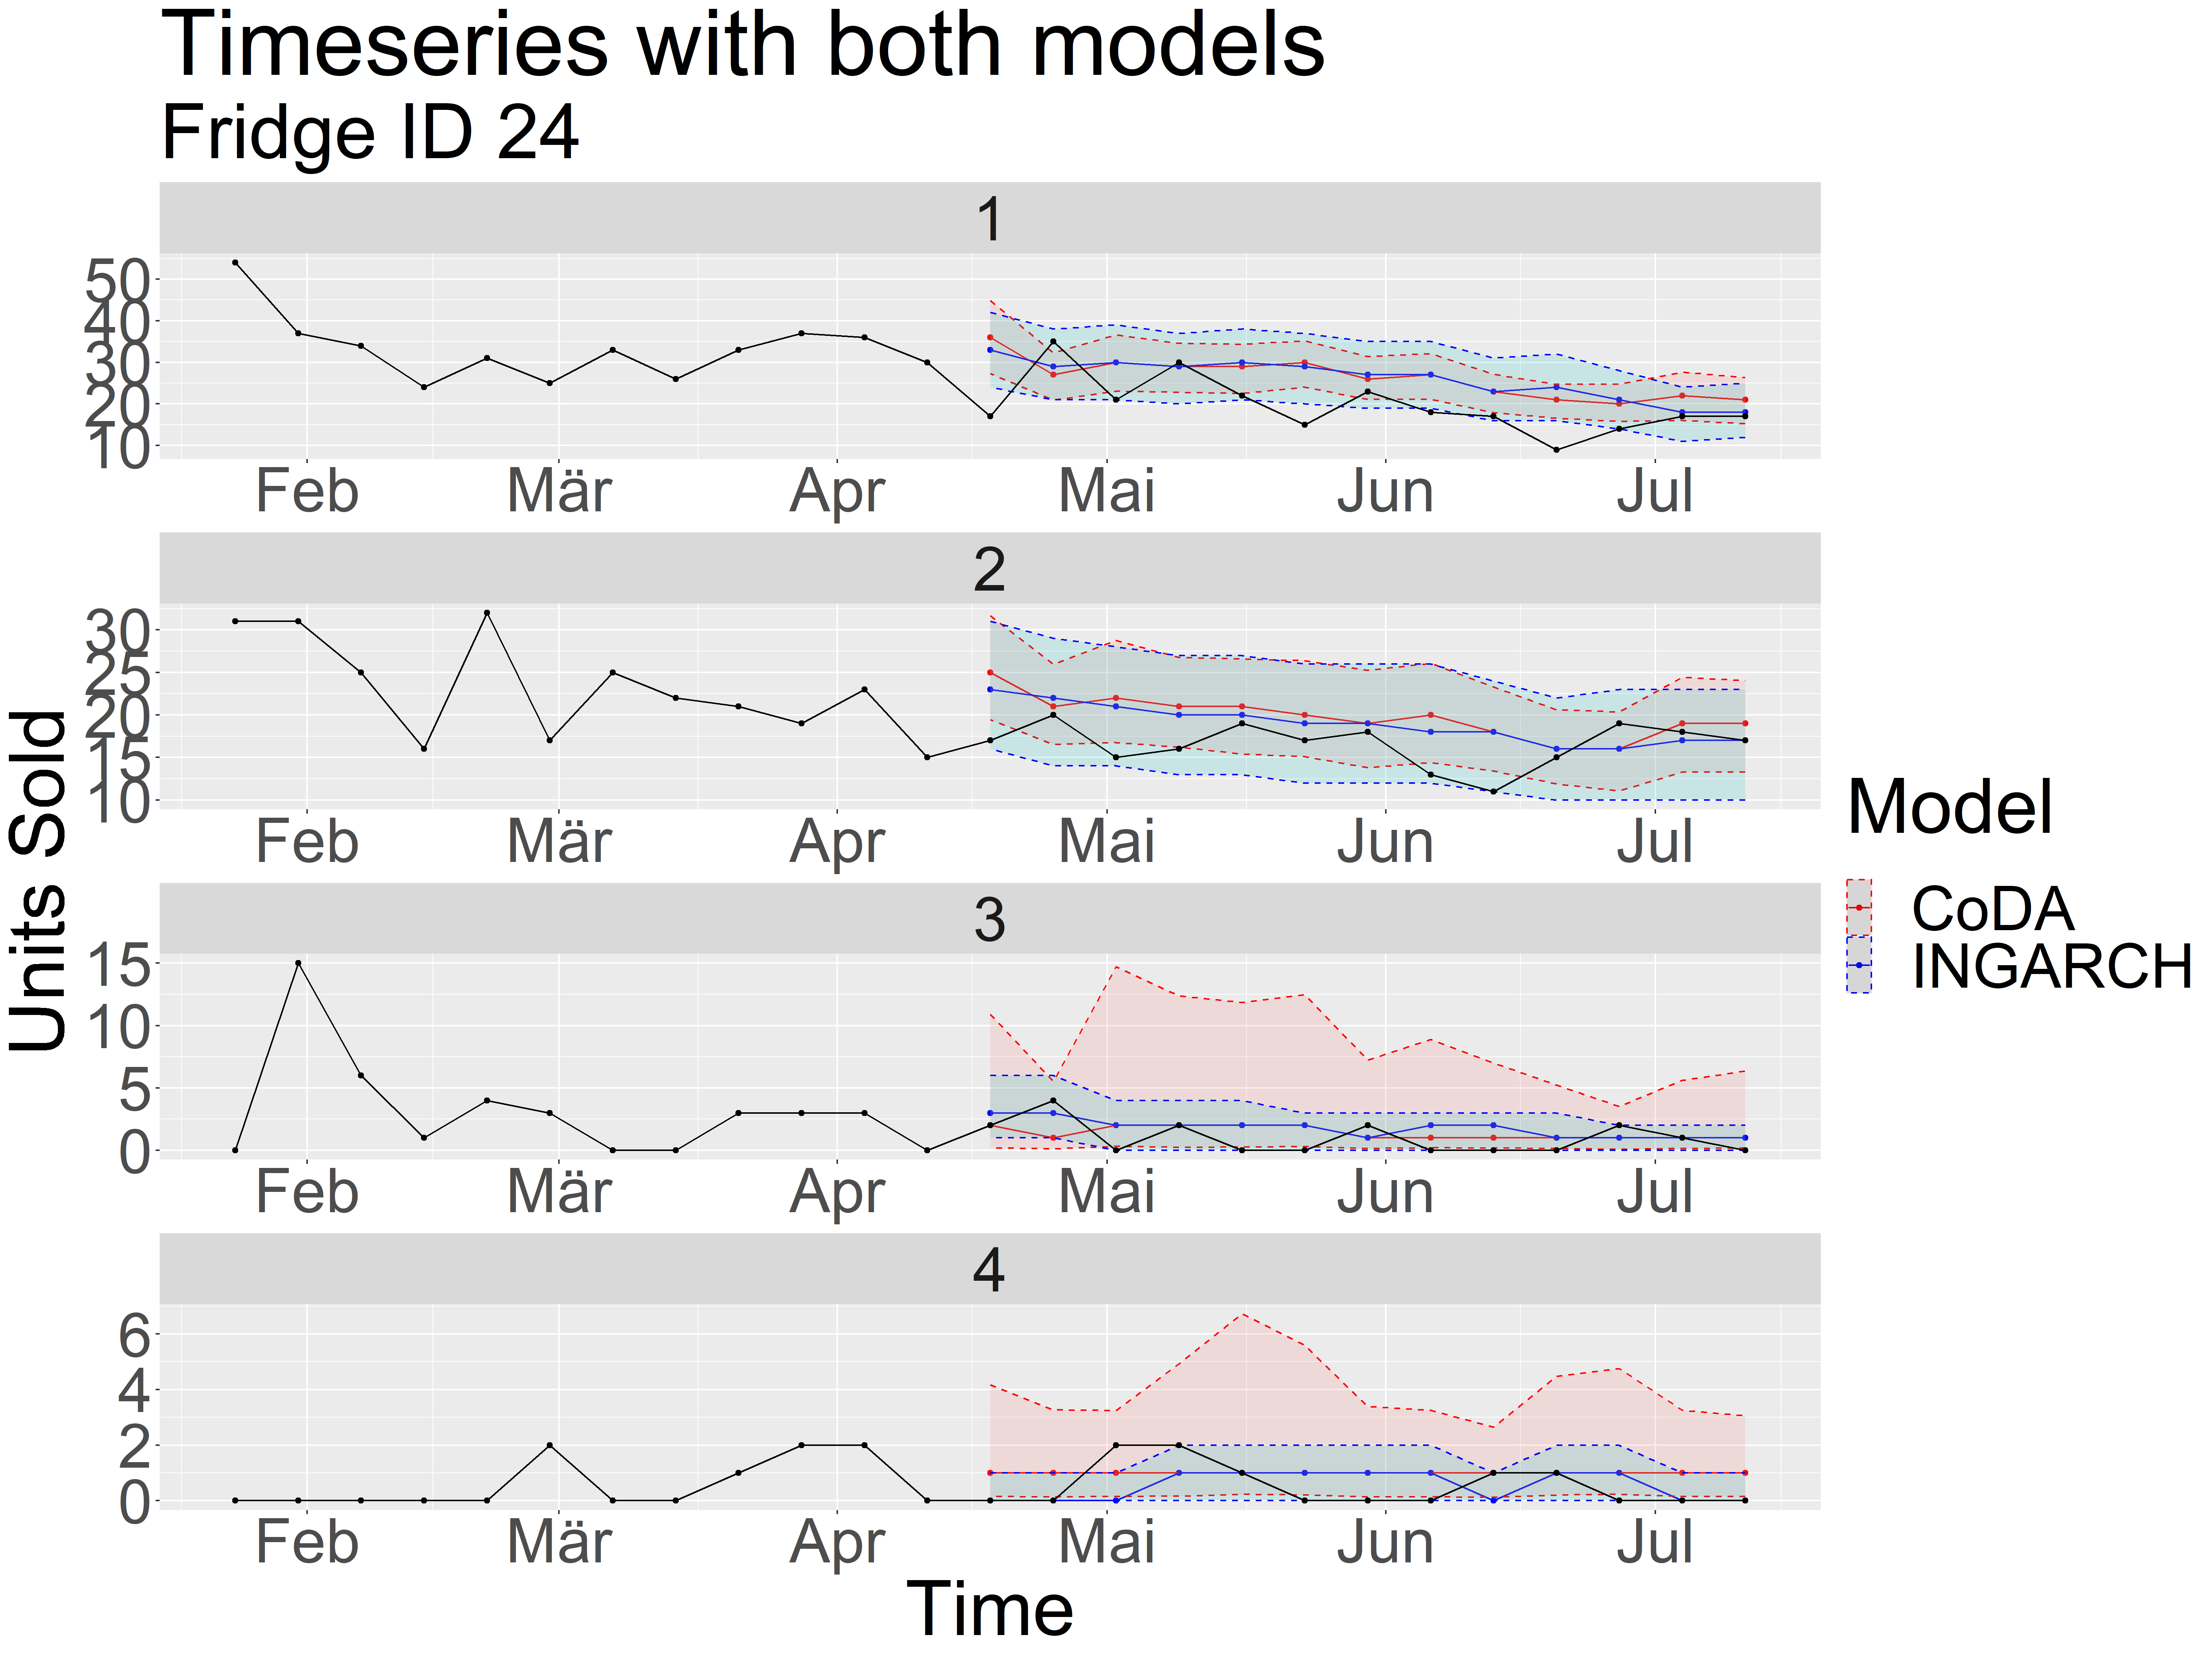
\includegraphics[width=\textwidth]{F:/Uni/Masterarbeit/Master-Thesis_git/Arbeit/Graphiken/BothPI_Timeseries_ID24.png}
\caption{Fridge 24 with the both models and their prediction intervals}
\label{fig:BothPI Fridge 24}
\end{subfigure}
\caption{Timeseries with both models and their prediction intervals}
\label{fig:TS BothPI}
\end{figure}
%%%%%%%%%%%%%%%%%%%%%%%%%%%%%%%%%%%%%%%%%%%%%%%%%%%%%%%%%%%%%
%% LITERATUR UND ANDERE VERZEICHNISSE
%%%%%%%%%%%%%%%%%%%%%%%%%%%%%%%%%%%%%%%%%%%%%%%%%%%%%%%%%%%%%

\addtocontents{toc}{\protect\vspace*{\baselineskip}}

%% Literaturverzeichnis
\printbibliography

%% Abbildungsverzeichnis
\clearpage
\addcontentsline{toc}{chapter}{List of Figures}
\listoffigures

%% Tabellenverzeichnis
\clearpage
\addcontentsline{toc}{chapter}{List of Tables}
\listoftables


%%%%%%%%%%%%%%%%%%%%%%%%%%%%%%%%%%%%%%%%%%%%%%%%%%%%%%%%%%%%%
%% ANHÄNGE
%%%%%%%%%%%%%%%%%%%%%%%%%%%%%%%%%%%%%%%%%%%%%%%%%%%%%%%%%%%%%
\appendix

\end{document}


